\documentclass[fleqn,10pt]{wlscirep}
%DIF LATEXDIFF DIFFERENCE FILE
%DIF DEL main_1.tex   Tue Jun 23 07:39:36 2020
%DIF ADD main_2.tex   Tue Jul  7 07:55:57 2020
\usepackage[utf8]{inputenc}
\usepackage[T1]{fontenc}
\usepackage{microtype}
\usepackage{algorithm}
\usepackage{algpseudocode}
%DIF 7a7
 %DIF > 
%DIF -------
\title{Cascades across networks are sufficient for the formation of echo chambers: An agent-based model}

\author[1*]{Jan-Philipp Fr{\"a}nken}
\author[2,3]{Toby D. Pilditch}


\affil[1]{Department of Psychology, University of Edinburgh, Edinburgh, EH8 9JZ, 7 George Square, United Kingdom}
\affil[2]{School of Geography and the Environment, University of Oxford, OX1 3QY, South Parks Road, Oxford, United
Kingdom}
\affil[3]{Department of Experimental Psychology, University College London, WC1H 0AP, 26 Bedford Way,
London, United Kingdom}

\affil[*]{Correspondence and requests for materials should be addressed to \href{mailto:jp.franken@ed.ac.uk}{jp.franken@ed.ac.uk}}

\keywords{social networks; echo chambers; source credibility; information cascades; agent-based modeling; Bayesian modeling}

\begin{abstract}
%DIF 24c25
%DIF < Investigating how echo chambers emerge in social networks is increasingly crucial, given their role in facilitating the retention of misinformation, inducing intolerance towards opposing views, and misleading public and political discourse (e.g., disbelief in climate change). Previously, the emergence of echo chambers has been attributed to psychological biases and inter-individual differences, requiring repeated interactions among network-users. In the present work we show that two core components of social networks---users self-select their networks, and information is shared laterally (i.e. peer-to-peer)---are causally sufficient to produce echo chambers. Crucially, we show that this requires neither special psychological explanation (e.g., bias or individual differences), nor repeated interactions---though these may be exacerbating factors. In fact, this effect is made increasingly worse the more generations of peer-to-peer transmissions it takes for information to permeate a network. This raises important questions for social network architects, if truly opposed to the increasing prevalence of deleterious societal trends that stem from echo chamber formation.
%DIF -------
Investigating how echo chambers emerge in social networks is increasingly crucial, given their role in facilitating the retention of misinformation, inducing intolerance towards opposing views, and misleading public and political discourse (e.g., disbelief in climate change). Previously, the emergence of echo chambers has been attributed to psychological biases and inter-individual differences, requiring repeated interactions among network-users. Using an idealised population of social network users, the present results suggest that two core components of social networks---users self-select their networks, and information is shared laterally (i.e. peer-to-peer)---might be causally sufficient to produce echo chambers. Crucially, we show that this requires neither special psychological explanation (e.g., bias or individual differences), nor repeated interactions---though these may be exacerbating factors. In fact, this effect is made increasingly worse the more generations of peer-to-peer transmissions it takes for information to permeate a network. This raises important questions for social network architects, if truly opposed to the increasing prevalence of deleterious societal trends that stem from echo chamber formation. %DIF > 
%DIF -------
\end{abstract}
%DIF PREAMBLE EXTENSION ADDED BY LATEXDIFF
%DIF UNDERLINE PREAMBLE %DIF PREAMBLE
\RequirePackage[normalem]{ulem} %DIF PREAMBLE
\RequirePackage{color}\definecolor{RED}{rgb}{1,0,0}\definecolor{BLUE}{rgb}{0,0,1} %DIF PREAMBLE
\providecommand{\DIFadd}[1]{{\protect\color{blue}\uwave{#1}}} %DIF PREAMBLE
\providecommand{\DIFdel}[1]{{\protect\color{red}\sout{#1}}}                      %DIF PREAMBLE
%DIF SAFE PREAMBLE %DIF PREAMBLE
\providecommand{\DIFaddbegin}{} %DIF PREAMBLE
\providecommand{\DIFaddend}{} %DIF PREAMBLE
\providecommand{\DIFdelbegin}{} %DIF PREAMBLE
\providecommand{\DIFdelend}{} %DIF PREAMBLE
\providecommand{\DIFmodbegin}{} %DIF PREAMBLE
\providecommand{\DIFmodend}{} %DIF PREAMBLE
%DIF FLOATSAFE PREAMBLE %DIF PREAMBLE
\providecommand{\DIFaddFL}[1]{\DIFadd{#1}} %DIF PREAMBLE
\providecommand{\DIFdelFL}[1]{\DIFdel{#1}} %DIF PREAMBLE
\providecommand{\DIFaddbeginFL}{} %DIF PREAMBLE
\providecommand{\DIFaddendFL}{} %DIF PREAMBLE
\providecommand{\DIFdelbeginFL}{} %DIF PREAMBLE
\providecommand{\DIFdelendFL}{} %DIF PREAMBLE
%DIF LISTINGS PREAMBLE %DIF PREAMBLE
\RequirePackage{listings} %DIF PREAMBLE
\RequirePackage{color} %DIF PREAMBLE
\lstdefinelanguage{DIFcode}{ %DIF PREAMBLE
%DIF DIFCODE_UNDERLINE %DIF PREAMBLE
  moredelim=[il][\color{red}\sout]{\%DIF\ <\ }, %DIF PREAMBLE
  moredelim=[il][\color{blue}\uwave]{\%DIF\ >\ } %DIF PREAMBLE
} %DIF PREAMBLE
\lstdefinestyle{DIFverbatimstyle}{ %DIF PREAMBLE
	language=DIFcode, %DIF PREAMBLE
	basicstyle=\ttfamily, %DIF PREAMBLE
	columns=fullflexible, %DIF PREAMBLE
	keepspaces=true %DIF PREAMBLE
} %DIF PREAMBLE
\lstnewenvironment{DIFverbatim}{\lstset{style=DIFverbatimstyle}}{} %DIF PREAMBLE
\lstnewenvironment{DIFverbatim*}{\lstset{style=DIFverbatimstyle,showspaces=true}}{} %DIF PREAMBLE
%DIF END PREAMBLE EXTENSION ADDED BY LATEXDIFF

\begin{document}

\flushbottom
\maketitle
% * <john.hammersley@gmail.com> 2015-02-09T12:07:31.197Z:
%
%  Click the title above to edit the author information and abstract
%
\thispagestyle{empty}


As we navigate social media platforms, we are free to customise our networks according to our individual needs: we choose to connect with users we like while we ignore others, we follow `Influencers' that inspire us, and we selectively share and repost content. Combined with curated News Feeds, selective attention to and sharing of content has been associated with spreading of digital misinformation \cite{del2016spreading} and false news stories \cite{vosoughi2018spread}. 
\DIFdelbegin \DIFdel{For example, it has been shown that people retweet false news stories more frequently than correct news stories, resulting in false rumour cascades on Twitter \mbox{%DIFAUXCMD
\cite{vosoughi2018spread, dizikes2018study}}\hspace{0pt}%DIFAUXCMD
. 
}%DIFDELCMD < 

%DIFDELCMD < %%%
\DIFdelend %DIF >  For example, it has been shown that people retweet false news stories more frequently than correct news stories, resulting in false rumour cascades on Twitter \cite{vosoughi2018spread, dizikes2018study}. 
Over the past decade, several researchers investigated the spreading and retention of misinformation and false news on social media platforms \cite{starbird2014rumors, bessi2015science, bakshy2015exposure, del2016spreading} and their implications for e.g., the polarisation of opinions \cite{bessi2016users, sikder2020minimalistic}. However, the scientific community still lacks clear answers to fundamental questions relating to \DIFdelbegin \DIFdel{1) }\DIFdelend the general prevalence of misinformation and false news \DIFdelbegin \DIFdel{\mbox{%DIFAUXCMD
\cite{lazer2018science} }\hspace{0pt}%DIFAUXCMD
and 2) }\DIFdelend \DIFaddbegin \DIFadd{and }\DIFaddend their effects on individuals \DIFdelbegin \DIFdel{. Consequently, the demand for research investigating how misinformation and false news are spread through social media remains an important topic. 
}\DIFdelend \DIFaddbegin \DIFadd{\mbox{%DIFAUXCMD
\cite{lazer2018science}}\hspace{0pt}%DIFAUXCMD
.
}\DIFaddend 

%DIF >  Consequently, the demand for research investigating how misinformation and false news are spread through social media remains an important topic. 
\DIFaddbegin 

\DIFaddend To understand the spreading of misinformation and false news, recent work has investigated the impact of echo chambers on digital misinformation. Echo chambers \DIFdelbegin \DIFdel{have been defined as }\DIFdelend \DIFaddbegin \DIFadd{are }\DIFaddend enclosed epistemic systems where like-minded individuals reinforce their pre-existing beliefs \cite{madsen2018large}. The enclosing nature of echo chambers has been shown to induce intolerance towards opposing views \cite{takikawa2017political}\DIFdelbegin \DIFdel{and }\DIFdelend \DIFaddbegin \DIFadd{, misleading public and political discourse \mbox{%DIFAUXCMD
\cite{jasny2015empirical, jasny2019echo} }\hspace{0pt}%DIFAUXCMD
and }\DIFaddend quantitative analyses suggest that echo chambers may contribute to the  spread of misinformation \cite{tornberg2018echo, del2016spreading}. 
\DIFdelbegin \DIFdel{Corroborating these findings, recent empirical research has shown that echo chambers lead to a misleading of public and political discourse, such as disbelief in climate change \mbox{%DIFAUXCMD
\cite{jasny2015empirical, jasny2019echo}}\hspace{0pt}%DIFAUXCMD
. }\DIFdelend %DIF >  Corroborating these findings, recent empirical research has shown that echo chambers lead to a misleading of public and political discourse, such as disbelief in climate change \cite{jasny2015empirical, jasny2019echo}. 
Investigating how echo chambers emerge on social media thus offers an important opportunity for understanding and potentially counteracting the occurrence of digital misinformation.

Importantly, although some social media users might `live' in echo chambers, using social media does not necessarily imply restricted exposure to information. Compared to non-users, the average social media user experiences more diverse content \cite{newman2017reuters} \DIFaddbegin \DIFadd{and it has been suggested that the majority of social media users do not necessarily self-select into echo chambers \mbox{%DIFAUXCMD
\cite{haw2020drives}}\hspace{0pt}%DIFAUXCMD
}\DIFaddend . Moreover, recent theoretical work \DIFdelbegin \DIFdel{suggests }\DIFdelend \DIFaddbegin \DIFadd{shows }\DIFaddend that echo chambers might improve individual access to information via \DIFdelbegin \DIFdel{optimizing }\DIFdelend \DIFaddbegin \DIFadd{optimising }\DIFaddend the allocation of information resources \cite{jann2018echo}. These findings further highlight the importance of clarifying how echo chambers emerge on social media, and raise questions about the value-free nature of echo-chambers. \DIFdelbegin \DIFdel{What factors lead to an echo-chamber causing harmful outcomes vs. beneficial ones? 
}\DIFdelend %DIF > What factors lead to an echo-chamber causing harmful outcomes vs. beneficial ones? 

In the present work, we formally study echo chamber formation within simulated populations of social media users. We expand the previous literature through two primary contributions, motivated by two important elements of social networks: 1) users are self-selecting in their peer networks (e.g., form connections based on friendship), and 2) users can share information rapidly in a peer-to-peer manner (i.e. lateral transmission). Specifically, we investigate the emergence of echo chambers as a result of a single pass-through of information prior to repeated interaction between users (contribution 1)\DIFdelbegin \DIFdel{. Moreover, we explore the impact of a social media }\DIFdelend \DIFaddbegin \DIFadd{, and how this is impacted by a }\DIFaddend user's perceived credibility of their peers \DIFdelbegin \DIFdel{on the formation of echo chambers }\DIFdelend (contribution 2). 

We test the robustness of these contributions across a wide range of network setups varying in terms of \DIFdelbegin \DIFdel{the }\DIFdelend epistemic authority (expertise strength) of users (robustness check 1), \DIFdelbegin \DIFdel{the }\DIFdelend percentage of users sharing their beliefs with their peers (robustness check 2), and their connectivity density (robustness check 3). Moreover, we contrast two \DIFdelbegin \DIFdel{different }\DIFdelend hypothetical populations of agents\DIFdelbegin \DIFdel{(see Methods for details)}\DIFdelend . For the first population (`social agents'), we assume that social media users select their network-peers based on whom they like (i.e. positive credibility). Conceptually, social agents are comparable to social media users that customise their networks based on positive perceptions of others (e.g., friendship). The second population (`asocial agents') functions as control check\DIFdelbegin \DIFdel{for the relevance of self-selection based on friendship / positive perceptions of others. Consequently, asocial agents select }\DIFdelend \DIFaddbegin \DIFadd{, selecting }\DIFaddend their network peers at random and independent of their perceived credibility. Given these considerations, we hope to \DIFdelbegin \DIFdel{further }\DIFdelend clarify the relationship between various conflated causes of echo chambers. 


\section*{Background and motivation}
\subsection*{Echo chambers}
To investigate when and how echo chambers emerge, it is important to explore their causes. These might be routed in psychological biases: previous analyses of echo chambers and their impact on digital misinformation identified confirmation bias---seeking information confirming one's prior beliefs \cite{nickerson1998confirmation}---and social influence---peoples' tendency to align their behaviour with the demands of their social environment \cite{kelman1958compliance}---as key driving factors of echo chamber formation
\cite{del2016spreading, starnini2016emergence, sikder2020minimalistic}. \DIFdelbegin \DIFdel{Similarly, }\DIFdelend \DIFaddbegin \DIFadd{For example, a recent quantitative analysis showed that social influence combined with a preference for forming connections with similar peers and abandoning dissimilar social ties results in rapid echo chamber formation after repeated interaction \mbox{%DIFAUXCMD
\cite{sasahara2019inevitability}}\hspace{0pt}%DIFAUXCMD
. Additionally, }\DIFaddend work in statistical physics has shown that confirmation bias induces clustering of like-minded individuals (i.e. echo chambers) and proliferation of opinions \cite{ngampruetikorn2016bias}. 

The above findings might be explained by the fact that \DIFdelbegin \DIFdel{confirmation bias leads }\DIFdelend \DIFaddbegin \DIFadd{social influence and confirmation bias lead }\DIFaddend to selective avoidance of information challenging one's prior beliefs, and consequently, limited access to cross-cutting content on social media such as Facebook \DIFdelbegin \DIFdel{\mbox{%DIFAUXCMD
\cite{bakshy2015exposure, ngampruetikorn2016bias}}\hspace{0pt}%DIFAUXCMD
}\DIFdelend \DIFaddbegin \DIFadd{\mbox{%DIFAUXCMD
\cite{henry2011emergence, bakshy2015exposure, ngampruetikorn2016bias}}\hspace{0pt}%DIFAUXCMD
}\DIFaddend . Along with psychological biases, it has also been argued that cognitive differences between individuals might induce echo chambers \cite{barkun2013culture}. Overall, these findings suggest that both psychological variables and cognitive variability among individual agents might be necessary requirements for the formation of echo chambers.

Aiming to clarify the necessity of psychological variables and heterogeneity, recent simulation-based work has investigated echo chamber formation in an idealised population of homogeneous rational (i.e. Bayesian) agents engaging in repeated interaction \DIFaddbegin \DIFadd{and with a preference for similar-minded others }\DIFaddend \cite{madsen2018large, madsen2017growing}. Results provided a formal argument for the inherent susceptibility of social networks towards echo chamber formation despite \emph{absence} of cognitive differences among agents. In other words, the \DIFdelbegin \DIFdel{findings of \mbox{%DIFAUXCMD
\cite{madsen2018large} }\hspace{0pt}%DIFAUXCMD
suggest that the }\DIFdelend \textit{structure} of social networks\DIFdelbegin \DIFdel{alone }\DIFdelend \DIFaddbegin \DIFadd{, in conjunction with a bias against dissimilar peers, }\DIFaddend is sufficient for the formation of echo chambers. \DIFaddbegin \DIFadd{These findings are in line with earlier work showing echo chambers inevitably emerge if users engaging in repeated interaction preferentially rewire their social ties to avoid contact with dissimilar peers \mbox{%DIFAUXCMD
\cite{henry2011emergence}}\hspace{0pt}%DIFAUXCMD
. 
}\DIFaddend 

Importantly, while previous work on echo chambers \cite{madsen2018large, madsen2017growing} and opinion dynamics (see also \cite{lorenz2007continuous}) \DIFdelbegin \DIFdel{already }\DIFdelend shows that repeated interaction solidifies echo chambers, the present work investigates whether the initial way in which information arrives into the network already `skews the pitch'. This is motivated by theoretical  \cite{bikhchandani1992theory} and simulation-based \cite{pilditch2017opinion} work on information cascades, which \DIFdelbegin \DIFdel{showed }\DIFdelend \DIFaddbegin \DIFadd{has shown }\DIFaddend that single interactions \DIFaddbegin \DIFadd{between equally rational agents }\DIFaddend can result in maladaptive \DIFdelbegin \DIFdel{collective }\DIFdelend outcomes prior to repeated interaction, and \DIFdelbegin \DIFdel{despite individually rational agents. Consequently, a single pass-through of information between generations of agents that update their beliefs sequentially might suffice for the emergence of echo chambers}\DIFdelend \DIFaddbegin \DIFadd{thus in the absence of rewiring of social ties}\DIFaddend . In other words, the connective density of social networks---including lateral transmission of information and limited access to the knowledge of the entire network---may be sufficient for echo chamber formation, even before repeated interaction, and without recourse to cognitive differences / \DIFdelbegin \DIFdel{biased explanations}\DIFdelend \DIFaddbegin \DIFadd{biases against forming social ties with users entertaining different beliefs}\DIFaddend . 

To investigate this we employed an agent-based model (in line with prior research on related phenomena \cite{madsen2017growing, madsen2018large}) that allowed us to simulate whether echo chambers emerge \DIFdelbegin \DIFdel{in social }\DIFdelend \DIFaddbegin \DIFadd{among }\DIFaddend agents as a consequence of \DIFdelbegin \DIFdel{social }\DIFdelend network structure (i.e. connective density---what percentage of the network is any given user \textit{directly} connected to?) in the \emph{absence} of repeated interaction (contribution 1). 
\DIFdelbegin \DIFdel{Specifically, we focused on a single cascade, meaning that all agents updated their beliefs sequentially through a single interaction. This method additionally allowed us }\DIFdelend %DIF >  Specifically, we focused on a single cascade, meaning that all agents updated their beliefs sequentially through a single interaction. 
\DIFaddbegin \DIFadd{As agents in our simulations were furnished with a homogeneous cognitive architecture, forming beliefs normatively through Bayesian updating, we were able }\DIFaddend to isolate structural aspects of a network from psychological variables and inter-individual differences among agents. 
\DIFdelbegin \DIFdel{Therefore, agents in our simulations were furnished with a homogeneous cognitive architecture, forming beliefs normatively through Bayesian updating. 
}\DIFdelend 

\subsection*{Source credibility}
The credibility of a source plays an important role when integrating their beliefs with our own observations and prior expectations \cite{cuddy2011dynamics, fiske2007universal}. Moreover, source credibility plays a critical role in persuasion and argumentation theory, especially in the context of politics \cite{housholder2014facebook, robinson1999measures, cialdini1993influence}, which has become increasingly influenced by online communication systems such as Facebook \cite{bail2016combining}. Both heuristic accounts, such as the heuristic-systematic model (HSM) \cite{chaiken1999heuristic} and dual-process theories, including the elaboration-likelihood model (ELM) \cite{petty1986elaboration} have been used to study the influence of credibility on persuasion, showing a positive general impact  \DIFdelbegin \DIFdel{of credibility on persuasion \mbox{%DIFAUXCMD
\cite{chaiken1994heuristic}}\hspace{0pt}%DIFAUXCMD
that has been extended to specific domains such as exercise intentions \mbox{%DIFAUXCMD
\cite{jones2003effects}}\hspace{0pt}%DIFAUXCMD
.}\DIFdelend \DIFaddbegin \DIFadd{\mbox{%DIFAUXCMD
\cite{chaiken1994heuristic}}\hspace{0pt}%DIFAUXCMD
.%DIF >  that has been extended to specific domains such as exercise intentions \cite{jones2003effects}. 
}\DIFaddend 

\DIFdelbegin \DIFdel{More recently}\DIFdelend \DIFaddbegin \DIFadd{Recently}\DIFaddend , research has investigated the influence of source credibility from a Bayesian perspective, meaning that credibility is modeled as an analytic cue \DIFdelbegin \DIFdel{influencing the probability of accepting a message / updating a belief }\DIFdelend \DIFaddbegin \DIFadd{that moderates belief updating }\DIFaddend \cite{bovens2003bayesian, hahn2009argument, harris2009bayesian, oaksford2007bayesian}. \DIFdelbegin \DIFdel{The Bayesian account provides }\DIFdelend \DIFaddbegin \DIFadd{This Bayesian Source Credilility model (BSCM) moves beyond previous models by providing }\DIFaddend a quantitative, normative framework for \DIFdelbegin \DIFdel{modeling }\DIFdelend \DIFaddbegin \DIFadd{modelling }\DIFaddend belief updating under consideration of the influence of credibility\DIFdelbegin \DIFdel{, which is a key advantage over alternative models such as ELM and HSM where the credibility of sources is conceptualised as a heuristic cue which does not allow for a quantitative formalisation}\DIFdelend . Empirical work supports the suitability of Bayesian representations of belief formation and credibility (see e.g., \cite{harris2016appeal}). \DIFdelbegin \DIFdel{Due }\DIFdelend \DIFaddbegin \DIFadd{Expanding on previous simulation work \mbox{%DIFAUXCMD
\cite{madsen2017growing, madsen2018large}}\hspace{0pt}%DIFAUXCMD
, and due }\DIFaddend to the quantitative nature of our analysis, we \DIFdelbegin \DIFdel{make use of the Bayesian credibility account, expanding previous simulation work \mbox{%DIFAUXCMD
\cite{madsen2017growing, madsen2018large} }\hspace{0pt}%DIFAUXCMD
through a measure of the credibility of a source }\DIFdelend \DIFaddbegin \DIFadd{deploy a BSCM account }\DIFaddend (i.e. an agent / social media user) \DIFdelbegin \DIFdel{in }\DIFdelend \DIFaddbegin \DIFadd{within }\DIFaddend our model (contribution 2). 
\DIFdelbegin \DIFdel{The next section introduces the details of our agent-based model.
}\DIFdelend %DIF >  The next section introduces the details of our agent-based model.


\section*{Model design and Simulations}

\subsection*{Agent-based models}
Agent-based models (ABMs) are simulated multi-agent systems that provide a formal framework for studying cognitive functions and behaviours in social environments---such as social media---which involve complex and dynamic interactions between users \cite{wilensky2015introduction}. Of particular relevance for our work is the advantage that ABMs allow for the capturing of emergent phenomena on a network level which is not possible when studying individual users in isolation from their peers  \cite{madsen2019analytic}. The advantages of ABMs for the study of complex and dynamic systems have been \DIFdelbegin \DIFdel{leveraged in several related studies, including ABMs of }\DIFdelend \DIFaddbegin \DIFadd{shown in research on }\DIFaddend belief formation in the context of climate change \cite{lewandowsky2019influence} and micro-targeting \cite{madsen2018method}. \DIFdelbegin \DIFdel{A full discussion of ABMs and their advantages for the study of dynamic systems and emergent phenomena is beyond the scope of the present contribution. }\DIFdelend In the remainder of this paper, we will \DIFdelbegin \DIFdel{therefore only }\DIFdelend refer to aspects of ABMs that are relevant to our model. \DIFdelbegin \DIFdel{Further details about ABMs and }\DIFdelend \DIFaddbegin \DIFadd{For further details on how to use ABMs and an elaborate discussion of }\DIFaddend their general advantages \DIFdelbegin \DIFdel{can be found elsewhere \mbox{%DIFAUXCMD
\cite{macal2005tutorial, madsen2019analytic}}\hspace{0pt}%DIFAUXCMD
.
}\DIFdelend \DIFaddbegin \DIFadd{for modelling cognitive phenomena, see \mbox{%DIFAUXCMD
\cite{macal2005tutorial, madsen2019analytic}}\hspace{0pt}%DIFAUXCMD
.
}\DIFaddend 

\DIFdelbegin \DIFdel{The three central components of ABMs are agents, patches, and links. Agents are the actors, and in our social network they correspond to individual users. Agents were furnished with cognitive functions and possible behaviours, including attention (detecting public declarations of others), belief revision (updating a prior belief-state based on observing another agent’s belief), and declaration (commit to a belief using a decision rule).
All agents were furnished with the same cognitive functions and possible behaviours. Links represent edges between agents. In the present model, (bidirectional) links were employed to enable signaling of public belief declarations between agents, and thus represent the (social) network connections. Patches are the building blocks of the environment in which agents act, though not relevant to the current model, like agents, patches can change dynamically. They have been used to model, for example, fluctuations in fish stock at a specific location \mbox{%DIFAUXCMD
\cite{bailey2018computational}}\hspace{0pt}%DIFAUXCMD
. 
}%DIFDELCMD < 

%DIFDELCMD < %%%
\DIFdelend Here, we reconstructed an idealised social network similar to \cite{pilditch2017opinion, madsen2018large} in which users (i.e. agents) \DIFdelbegin \DIFdel{form binary beliefs }\DIFdelend \DIFaddbegin \DIFadd{were distributed randomly in a two-dimensional space forming social ties based on proximity, as measured by Euclidean distance (see Methods for details). Agents communicated binary beliefs to their peers and updated them }\DIFaddend through a single interaction. \DIFdelbegin \DIFdel{As such, our }\DIFdelend \DIFaddbegin \DIFadd{Binary beliefs in this case means that agents could either believe in a hypothesis---belief \(h\)---or not believe in a hypothesis---belief \(\neg h\). Conceptually, this can be thought as a group of people that either support a political candidate (\(h\)) or not support a political candidate (\(\neg h\)). 
}

\DIFadd{Our }\DIFaddend agent-based model (ABM) captured agents' social environment \DIFdelbegin \DIFdel{and }\DIFdelend \DIFaddbegin \DIFadd{(social ties with peers) and the }\DIFaddend temporal dynamics of belief change \DIFaddbegin \DIFadd{(updating beliefs through interaction)}\DIFaddend , which both form necessary requirements for the observation of echo chambers. Additionally, our ABM accounted for heterogeneity between individual agents (such as different prior beliefs)\DIFdelbegin \DIFdel{, which is an important general }\DIFdelend \DIFaddbegin \DIFadd{; an }\DIFaddend advantage of agent-based simulations \cite{wilensky2015introduction}. \DIFdelbegin \DIFdel{Put another way}\DIFdelend \DIFaddbegin \DIFadd{Specifically}\DIFaddend , though we designed agents such that their cognitive \textit{functions} are the same \DIFaddbegin \DIFadd{(homogeneous cognitive architecture)}\DIFaddend , we allowed for the diversity among agents of particular belief \textit{values} \DIFdelbegin \DIFdel{.
}\DIFdelend \DIFaddbegin \DIFadd{(heterogeneous prior beliefs): Each agent was furnished with their own subjective prior beliefs, randomly sampled from a Gaussian distribution. As such, each agent had a unique prior belief about whether they would support a hypothesis or not. Thinking about a group of people again, this means that while they would all share the same mechanism (i.e., process) for updating their beliefs (homogeneous cognitive architecture), each of them would enter a discussion with their own subjective prior opinion (heterogeneous prior beliefs).
}\DIFaddend 

\DIFaddbegin \begin{figure}[ht]
\centering
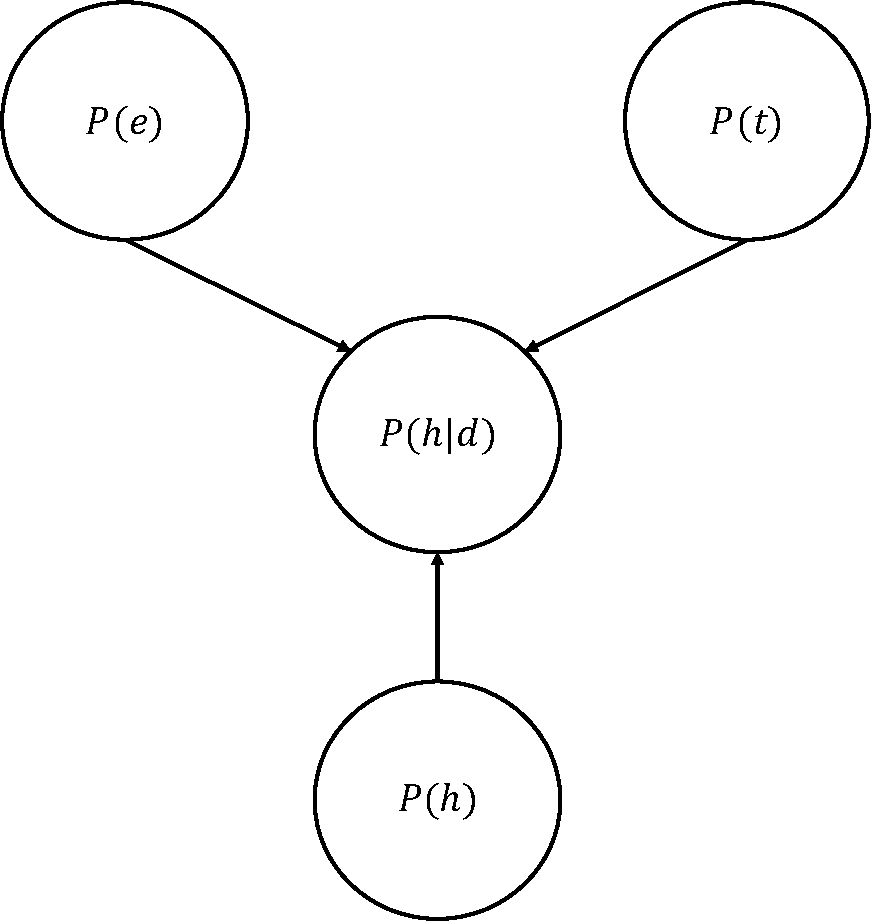
\includegraphics[width=0.35\columnwidth]{figure1.pdf}
\caption{\DIFaddFL{Figure shows how a prior belief \(P(h)\) and the perceived credibility of a source (operationalised via expertise \(P(e)\) and trustworthiness \(P(t)\)) interact within the BSCM framework.}}
\label{fig:bscm}
\end{figure}

\DIFaddend \subsection*{Bayesian source credibility model}
Bayesian theories of reasoning and decision making propose that a person's prior belief in a hypothesis is represented as subjective probability \(P(h)\) taking values between 0 and 1 (see e.g., \cite{hahn2007rationality, oaksford2007bayesian}). Upon observing new data, \(d\), the Bayesian framework posits that the posterior probability of a hypothesis, \(P(h|d)\), is given by the \DIFdelbegin \DIFdel{normalized }\DIFdelend \DIFaddbegin \DIFadd{normalised }\DIFaddend product of the likelihood \(P(d|h)\) and the prior \(P(h)\):

\begin{equation}
    P(h|d) = \frac{P(d|h)P(h)}{\sum_{h'}P(d|h')P(h')}.
\end{equation}

As in \cite{madsen2017growing, madsen2018large}, we wanted to ensure that individual differences and psychological variables would not conflate with the impact of network structure on the formation of echo chambers. Consequently, all agents were idealised reasoners adhering to the principles of Bayesian updating. To include the credibility of a source, we used \DIFdelbegin \DIFdel{a }\DIFdelend \DIFaddbegin \DIFadd{the }\DIFaddend Bayesian source credibility model (BSCM) \cite{bovens2003bayesian, hahn2009argument, harris2009bayesian}. In the BSCM framework, credibility has two components, perceived expertise, \(P(e)\), and perceived trustworthiness, \(P(t)\) (see also \cite{harris2016appeal}). \DIFdelbegin \DIFdel{The perceived expertise of a source }\DIFdelend \DIFaddbegin \DIFadd{Perceived expertise }\DIFaddend refers to the probability of the source \DIFdelbegin \DIFdel{'s communicated belief being correct. The perceived trustworthiness of a communicating agent }\DIFdelend \DIFaddbegin \DIFadd{having accurate information, whilst the perceived trustworthiness }\DIFaddend refers to the communicator's intention to \DIFdelbegin \DIFdel{tell the truth. In other words, \(P(t)\) can be thought of as what the communicator believes to be true, independent of whether the belief is correct or not}\DIFdelend \DIFaddbegin \DIFadd{pass on accurate information (to the best of their ability)}\DIFaddend . \(P(e)\) and \(P(t)\) (which are orthogonal in BSCM) are both incorporated within the belief revision process of the present agent-based model (see Fig. \ref{fig:bscm}).

\DIFdelbegin %DIFDELCMD < \begin{figure}[ht]
%DIFDELCMD < \centering
%DIFDELCMD < 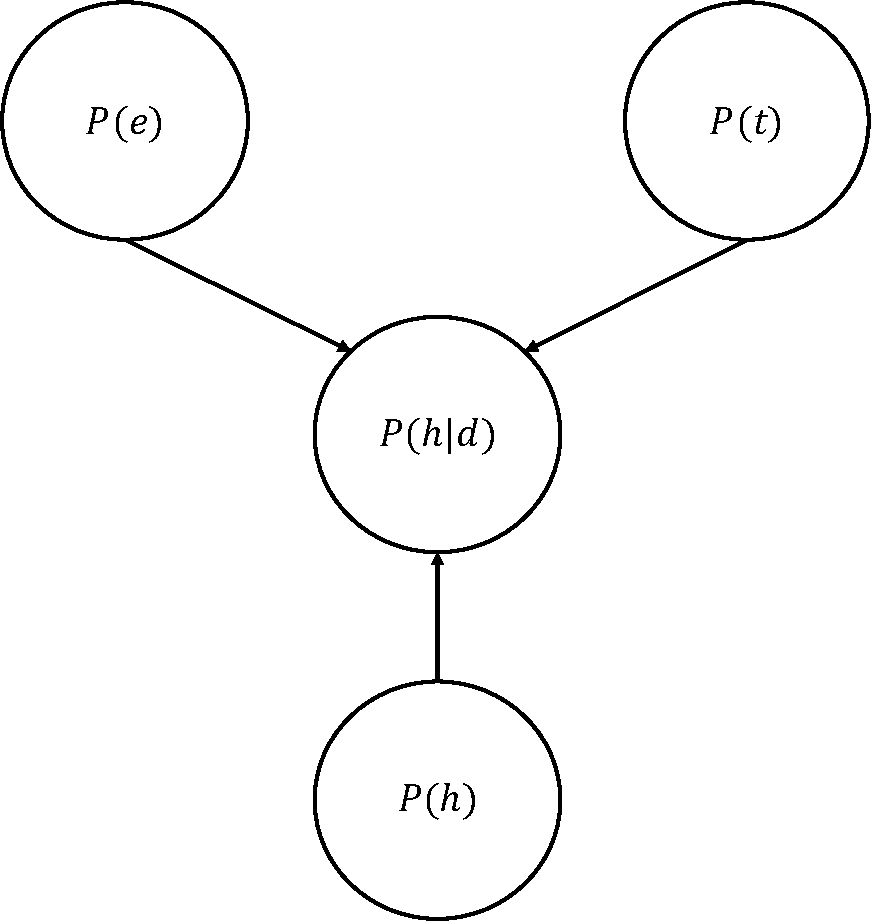
\includegraphics[width=0.4\columnwidth]{img/bscm_pdf.pdf}
%DIFDELCMD < %%%
%DIFDELCMD < \caption{%
{%DIFAUXCMD
\DIFdelFL{Figure shows how a prior belief \(P(h)\) and the perceived credibility of a source (operationalised via expertise \(P(e)\) and trustworthiness \(P(t)\)) interact within the BSCM framework.}}
%DIFAUXCMD
%DIFDELCMD < \label{fig:bscm}
%DIFDELCMD < \label{fig:bscm}
%DIFDELCMD < \end{figure}
%DIFDELCMD < 

%DIFDELCMD < %%%
\DIFdelend In the BSCM framework, the likelihood \DIFdelbegin \DIFdel{for an agent that }\DIFdelend \DIFaddbegin \DIFadd{that a communication target }\DIFaddend supports a hypothesis \(P(h)\) is given by\DIFaddbegin \DIFadd{:  
}\DIFaddend 

\begin{equation}
    P(d|h) = \sum_{e't'}P(h|e',t')P(e')P(t'). 
\end{equation}

In the same way, the likelihood for an agent that does not support a hypothesis \(P(\neg h)\) corresponds to

\begin{equation}
    P(d|\neg h) = \sum_{e't'}P(\neg h|e',t')P(e')P(t') 
\end{equation}

(see \cite{hahn2009argument, harris2016appeal} \DIFaddbegin \DIFadd{and Methods}\DIFaddend , for further details).  

The orthogonal nature of expertise and trust is typically operationalised such that trust being high or low leads to changes in the direction of belief revision (i.e. low trust makes you revise your beliefs in the opposite direction than high trust), whilst expertise moderates the strength (size) of the revision (see  \cite{bovens2003bayesian, harris2016appeal}). As a consequence, our manipulation of the perceived expertise strength, \(\textbf{\emph{e}}\), is a way to control how strongly a communication target is influenced by the \DIFdelbegin \DIFdel{expertise }\DIFdelend \DIFaddbegin \DIFadd{credibility }\DIFaddend of a source (robustness check 1; see Methods). Conceptually, expertise strength can be compared to epistemic authority (\DIFdelbegin \DIFdel{i.e. knowledge superiority; }\DIFdelend see also \cite{walton2010appeal})\DIFdelbegin \DIFdel{, which suggests that }\DIFdelend \DIFaddbegin \DIFadd{: }\DIFaddend a source with higher expertise \DIFdelbegin \DIFdel{strength }\DIFdelend is going to exert stronger influence on a receiver during belief revision. To explore \DIFdelbegin \DIFdel{the impact of knowledge superiority}\DIFdelend \DIFaddbegin \DIFadd{this}\DIFaddend , we investigated the influence of three \DIFdelbegin \DIFdel{different parameter settings for expertise strength }\DIFdelend \DIFaddbegin \DIFadd{expertise strength parameter settings }\DIFaddend on echo chamber formation (see Table \ref{tab:t1}). 


\subsection*{Simulations}
Agents were randomly assigned to x-y coordinates in a \DIFdelbegin \DIFdel{2-dimensional }\DIFdelend \DIFaddbegin \DIFadd{two-dimensional }\DIFaddend space, forming links with their nearest \DIFdelbegin \DIFdel{neighbors }\DIFdelend \DIFaddbegin \DIFadd{neighbours }\DIFaddend (refer to \cite{wilensky2015introduction}, for further details on how to spatially allocate agents in ABMs). Proximity was measured in terms of Euclidean distance, which has been used as a proxy for relational proximity in social networks \cite{duggins2017}. Prior to the start of a simulation, each agent sampled their own prior belief \(P(h)\) and subjective \(e\) and \(t\) values from univariate Gaussians with \(\mu\)=0.5 and \(\sigma^2\)=0.20 (for all three estimates, distributions were truncated between [0, 1]). Thus, \(P(h)\), \(e\), and \(t\) differed heterogeneously within our agent population. Following revision of their prior belief according to BSCM, agents declared for one of the two beliefs based on a deterministic decision rule: 

\[
Belief = \begin{cases}
h \text{ if } P(h|d) > 0.5 \\
\neg h \text{ if } P(h|d) < 0.5. 
\end{cases}
\]

If \(P(h|d)\) = 0.5, an agent declared either belief with a probability of 50\%. The declared belief (i.e. \(h\) or \(\neg h\)) was then made pubic based on the P(Declaration) probability (\DIFdelbegin \DIFdel{robustnes }\DIFdelend \DIFaddbegin \DIFadd{robustness }\DIFaddend check 2) which was manipulated between simulations (see Table \ref{tab:t1}). For example, a declaration of 1 means all agents made their beliefs public, while 0.10 means that there is a 10\% probability for each agent making their opinion public. The \DIFdelbegin \DIFdel{conceptual motivation for P(Declaration) }\DIFdelend \DIFaddbegin \DIFadd{motivation for inclusion }\DIFaddend is based on recent findings showing \DIFdelbegin \DIFdel{that }\DIFdelend \emph{most} social media users do not discuss their political beliefs on social media, but mainly focus on exchanging shared hobbies and passions \cite{newman2019reuters}. We wanted to ensure that our simulation results are robust across social networks varying in terms of the percentage of users discussing their beliefs with \DIFdelbegin \DIFdel{their }\DIFdelend peers. We thus explored \DIFdelbegin \DIFdel{the formation of echo chambers across }\DIFdelend three levels of P(Declaration) \DIFdelbegin \DIFdel{which can be thought of }\DIFdelend as a proxy for \DIFaddbegin \DIFadd{manipulating }\DIFaddend the percentage of people exchanging their beliefs about a particular topic (e.g., politics or news). 

\DIFdelbegin \DIFdel{In addition to P(Declaration)}\DIFdelend \DIFaddbegin \DIFadd{Lastly}\DIFaddend , we varied the connective density \DIFdelbegin \DIFdel{between simulations }\DIFdelend (i.e. what percentage of the overall network is any given user \textit{directly} connected to) from 0.5\% to 50.0\% (robustness check 3) \DIFaddbegin \DIFadd{between simulations}\DIFaddend . This allowed us to test whether the formation of echo chambers changes as a function of the number of `generations' it takes for information to \DIFdelbegin \DIFdel{pass across }\DIFdelend \DIFaddbegin \DIFadd{fully permeate }\DIFaddend a network (\DIFdelbegin \DIFdel{i.e.how many rounds of peer-to-peer communication to get across the }\DIFdelend \DIFaddbegin \DIFadd{e.g., 10\% connectivity means on average it will take 10 generations of communication to permeate the entire }\DIFaddend network). \DIFdelbegin \DIFdel{In this way, the }\DIFdelend \DIFaddbegin \DIFadd{The }\DIFaddend more links (connected friends / users) an agent has, the more \DIFdelbegin \DIFdel{likely the agent is to }\DIFdelend \DIFaddbegin \DIFadd{immediately an agent will }\DIFaddend see information appearing on the network \DIFdelbegin \DIFdel{early }\DIFdelend (and thus the shorter \DIFaddbegin \DIFadd{/ faster }\DIFaddend the cascade). This can \DIFdelbegin \DIFdel{also }\DIFdelend be compared to an \DIFdelbegin \DIFdel{increased number of }\DIFdelend friends on Facebook or followers on Twitter, where \DIFdelbegin \DIFdel{the information load of a user's News Feed increases if the person has more friends (Facebook) or follows more users (Twitter)}\DIFdelend \DIFaddbegin \DIFadd{higher numbers equates to a larger catchment of information coming in to the user}\DIFaddend . 


\begin{table}[ht]
\label{tab:robustness_checks}
\centering
\begin{tabular}{|l|l|l|}
\hline
Name & Description & Levels\\
\hline
Connectivity density (\%) & (Links per Agent / Total Number of Agents) \DIFdelbeginFL \DIFdelFL{* }\DIFdelendFL \DIFaddbeginFL \DIFaddFL{\(\times\) }\DIFaddendFL 100 & 0.5, 1.0, 1.5, ... 50.0\\
Expertise strength & Manipulating the magnitude of expertise \DIFdelbeginFL \DIFdelFL{influence }\DIFdelendFL \DIFaddbeginFL \DIFaddFL{strength }\DIFaddendFL (\(\textbf{\textit{e}}\)) & 0.00, 0.10, 0.20\\
P(Declaration) & Probability of making a belief public & 0.10, 0.50, 1.00\\
\hline
\end{tabular}
\caption{\label{tab:t1}Robustness checks.}
\end{table}


To measure echo chambers effectively across simulations, we were first interested in measuring global proportions of beliefs across the whole network (i.e. the relative number of agents with belief \(h\) compared to agents entertaining belief \(\neg h\)). Based on previous simulation-based work, we expected that global proportions would consistently approximate 50/50 across both agent populations \cite{pilditch2017opinion}. This measure was necessary to ensure that echo chambers are not a by-product of a dominant network-wide belief. Following checks for possible network-wide belief confounds, our key dependent measure of echo chamber formation was the average percentage of like-minded neighbours an agent possessed (i.e. the \textit{local} network similarity). \DIFdelbegin \DIFdel{This measure }\DIFdelend \DIFaddbegin \DIFadd{Specifically, measuring local network similarity allowed us to assess whether enclosed epistemic systems, which are a key component of echo chambers \mbox{%DIFAUXCMD
\cite{madsen2018large}}\hspace{0pt}%DIFAUXCMD
, formed during the simulations.
}


\DIFadd{Formally, local network similarity }\DIFaddend corresponded to the average percentage of agents in the target's direct network that shared the same belief as the target. For example, 50\% means that, on average, agents had equal proportions for each belief type in their direct network, where direct network refers to the fraction of the whole network that is directly connected to an agent. \DIFdelbegin %DIFDELCMD < 

%DIFDELCMD < %%%
\DIFdelend \DIFaddbegin \DIFadd{As such, a higher percentage of agents sharing the same belief as the target is a proxy for a more severe closure of the target's epistemic belief network, which means that it is less likely that the target will be confronted with a rebuttal (e.g., a user entertaining a different belief). }\DIFaddend In line with previous work \cite{pilditch2017opinion}, we expected that social agents would show increased percentages of like-minded neighbours (i.e. echo chambers) for low connectivity density values. We did not expect clustering effects in the asocial population in which agents selected network-peers at random \DIFdelbegin \DIFdel{and computed stochastic credibility estimates for a communicating source }\DIFdelend (see Methods for details).
\DIFdelbegin \DIFdel{Each system specification (connectivity density (100) x expertise strength (3) x P(Declaration) (3)) was ran independently 50 times, taking an average set of values for each specification. The total number of agents (n = 1000) was consistent across simulations. Simulations were conducted independently for each of the two agent populations.
}\DIFdelend 

\section*{Results}

Fig. \ref{fig:results} \DIFdelbegin \DIFdel{summarizes }\DIFdelend \DIFaddbegin \DIFadd{summarises }\DIFaddend our central findings. We predicted that for both social and asocial agents, global belief proportions would consistently approximate 50/50. Fig. \ref{fig:results}a (social agent population) and Fig. \ref{fig:results}b (asocial agent population) confirm these predictions. Specifically, Fig.  \ref{fig:results}a and \ref{fig:results}b show that global proportions of beliefs in both populations consistently approximated 50/50 irrespective of varying P(Declaration), connectivity density, or expertise strength. This finding is important, as it ensures that potential clusters of like-minded others (Fig. \ref{fig:results}c-d) do not result from a global bias towards either belief.

\DIFaddbegin \begin{figure}[ht]
\centering
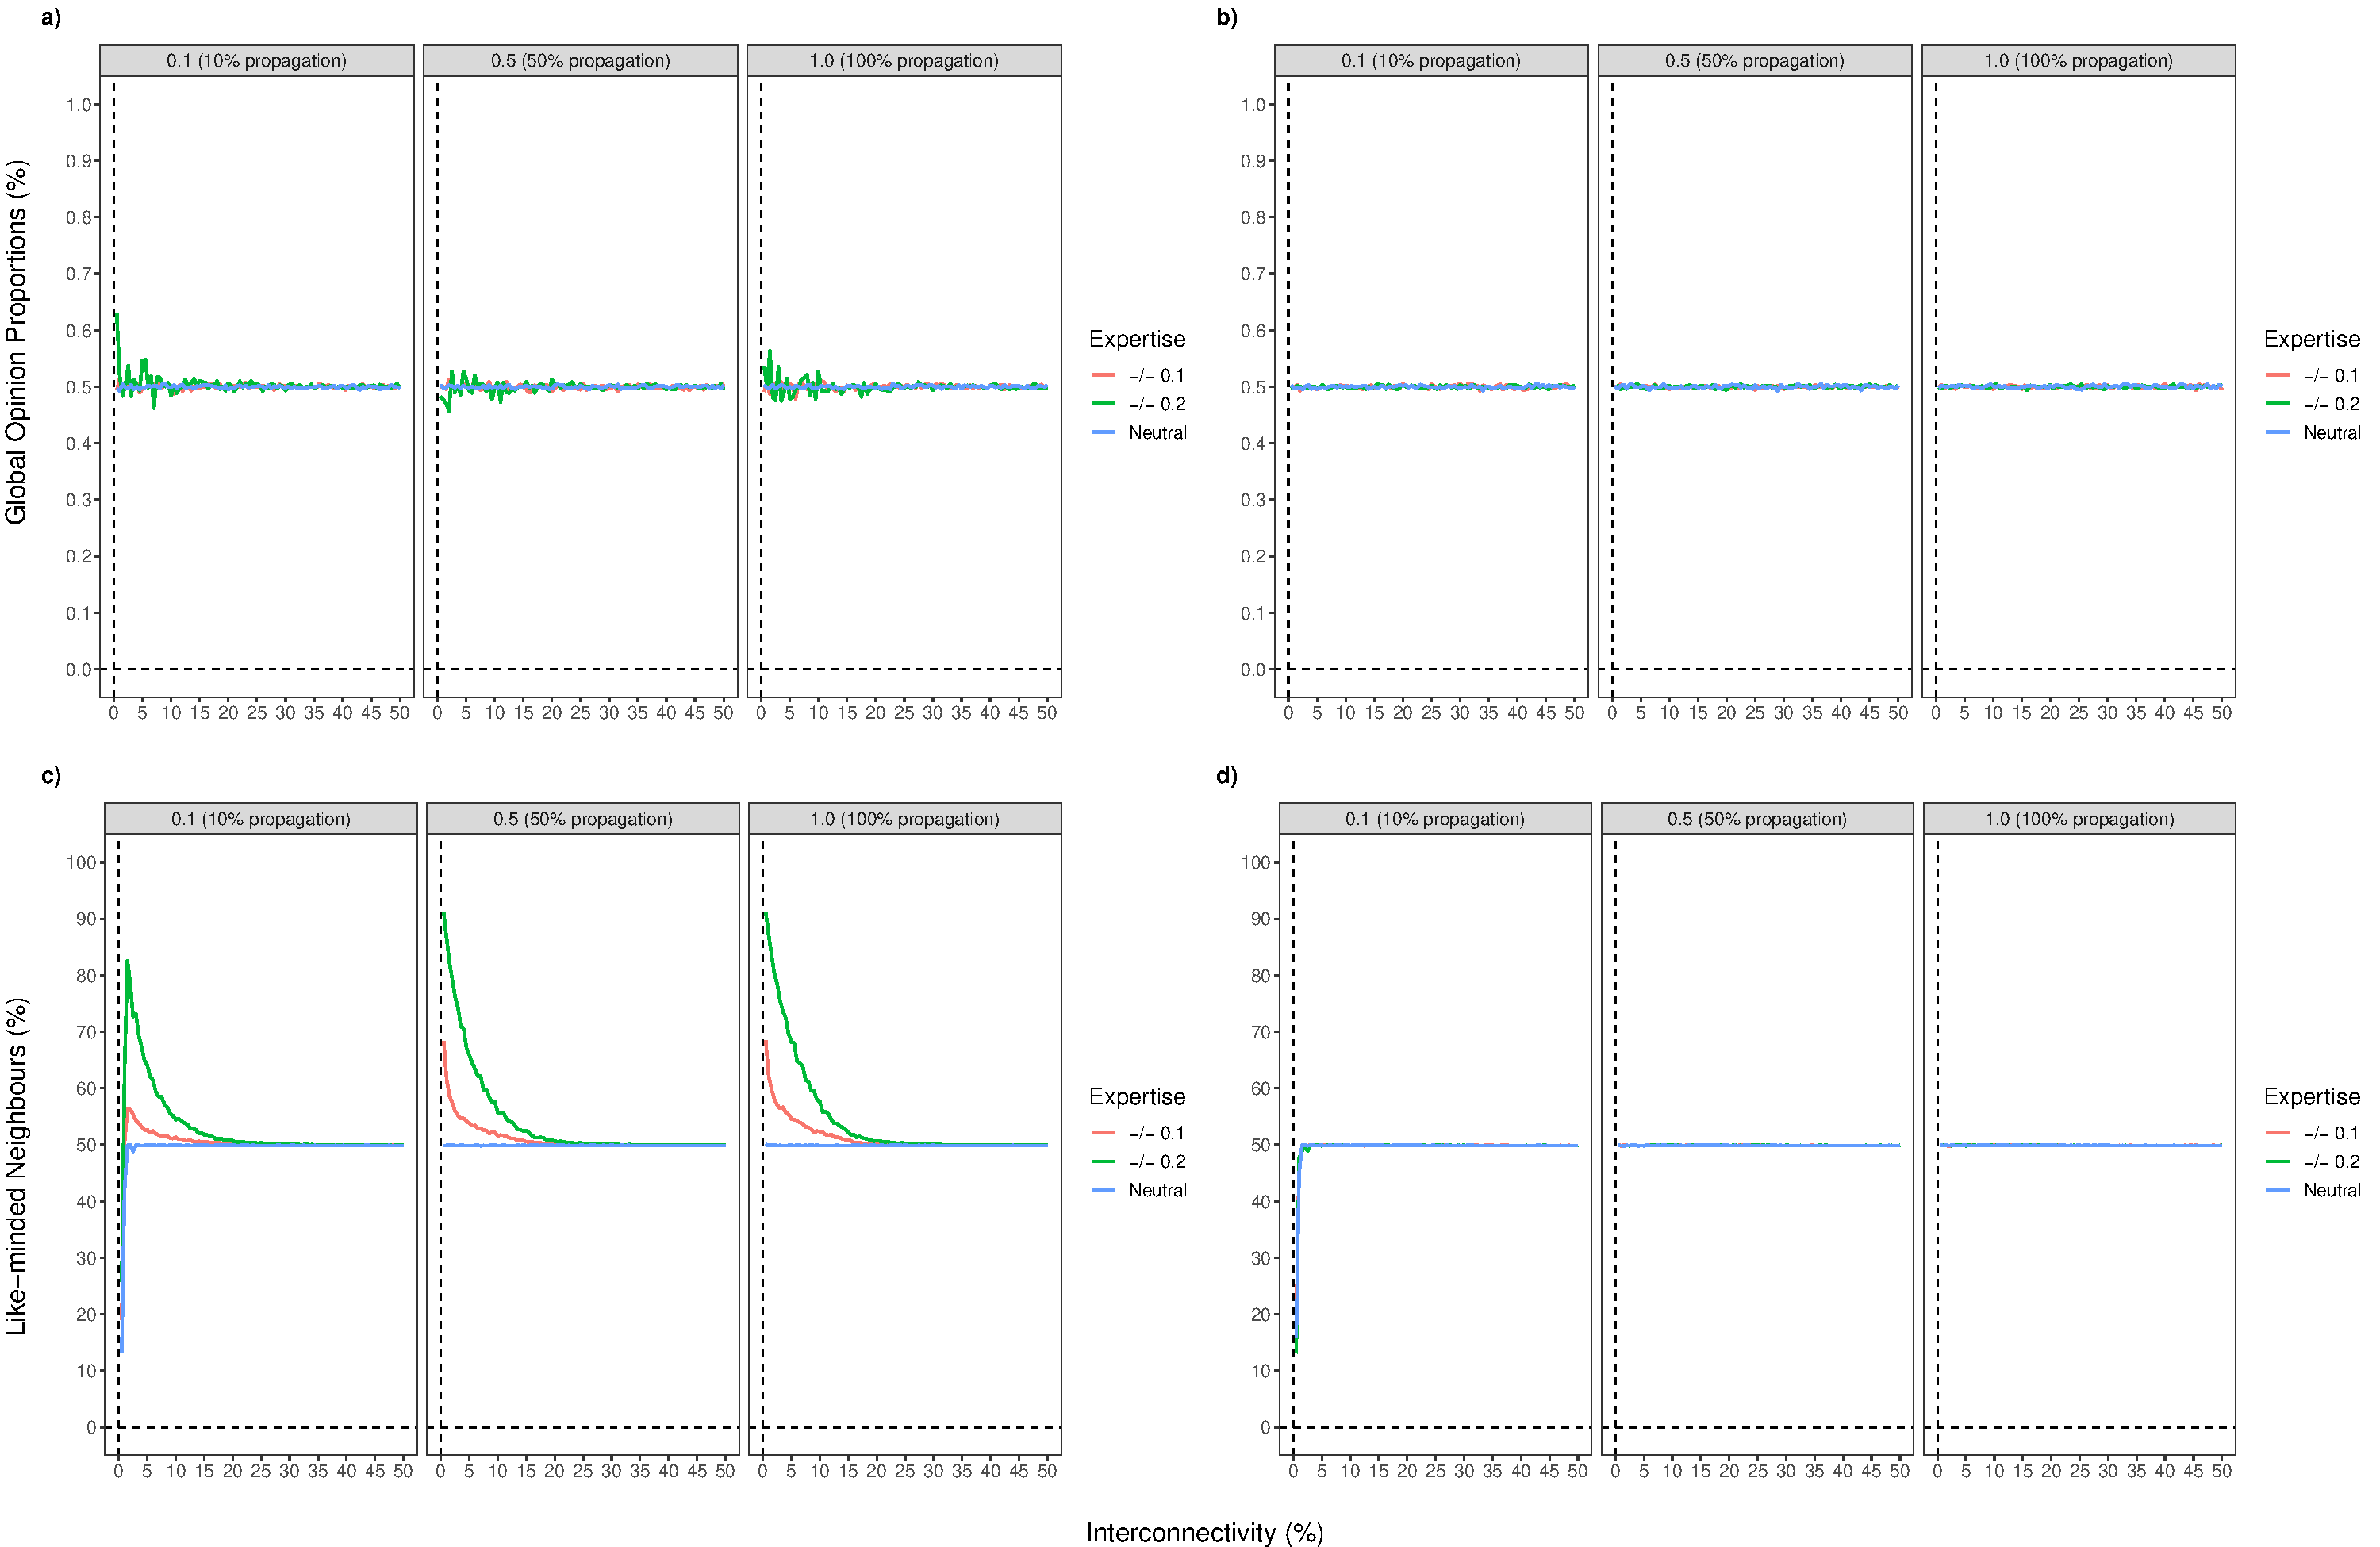
\includegraphics[width=1\columnwidth]{figure2.pdf}
\caption{\DIFaddFL{Main results. a) global belief proportions, social agents. b) global belief proportions, asocial agents. c) average percentage of like-minded neighbours (i.e. echo chambers), social agents. d) average percentage of like-minded neighbours (i.e. echo chambers), asocial agents.}}
\label{fig:results}
\end{figure}


\DIFaddend For social agents, the average proportion of like-minded \DIFdelbegin \DIFdel{neighbors }\DIFdelend \DIFaddbegin \DIFadd{neighbours }\DIFaddend (Fig. \ref{fig:results}c) increased as a function of increasing expertise strength, increasing P(Declaration) and decreasing connectivity density (x-axis). Importantly, to fully reduce the formation of echo chambers, the average network member must be connected to around 15-20\% of the network, which is infeasible considering the size of real world social networks which can have several Billion users. \DIFdelbegin \DIFdel{Our results }\DIFdelend \DIFaddbegin \DIFadd{The reason for a reduced clustering effect given increased connectivity density is that increasing connectivity density increases agents' access to information across the network (i.e. the beliefs of other agents). Thus, after reaching a connectivity density of around 15-20\%, each agents had access to a significant proportion of the beliefs across the entire network, which reduced the formation of epistemic circles isolated from opposing beliefs. Overall, our results showing a negative influence of increased connectivity density on echo chamber formation }\DIFaddend are comparable to previous simulation-based work exploring echo \DIFdelbegin \DIFdel{chamber formation in a a }\DIFdelend \DIFaddbegin \DIFadd{chambers in a }\DIFaddend population of stochastic reinforcement learners \cite{pilditch2017opinion}\DIFdelbegin \DIFdel{, although the present findings revealed less intense clustering effects}\DIFdelend . 


\DIFdelbegin %DIFDELCMD < \begin{figure}[ht]
%DIFDELCMD < \centering
%DIFDELCMD < 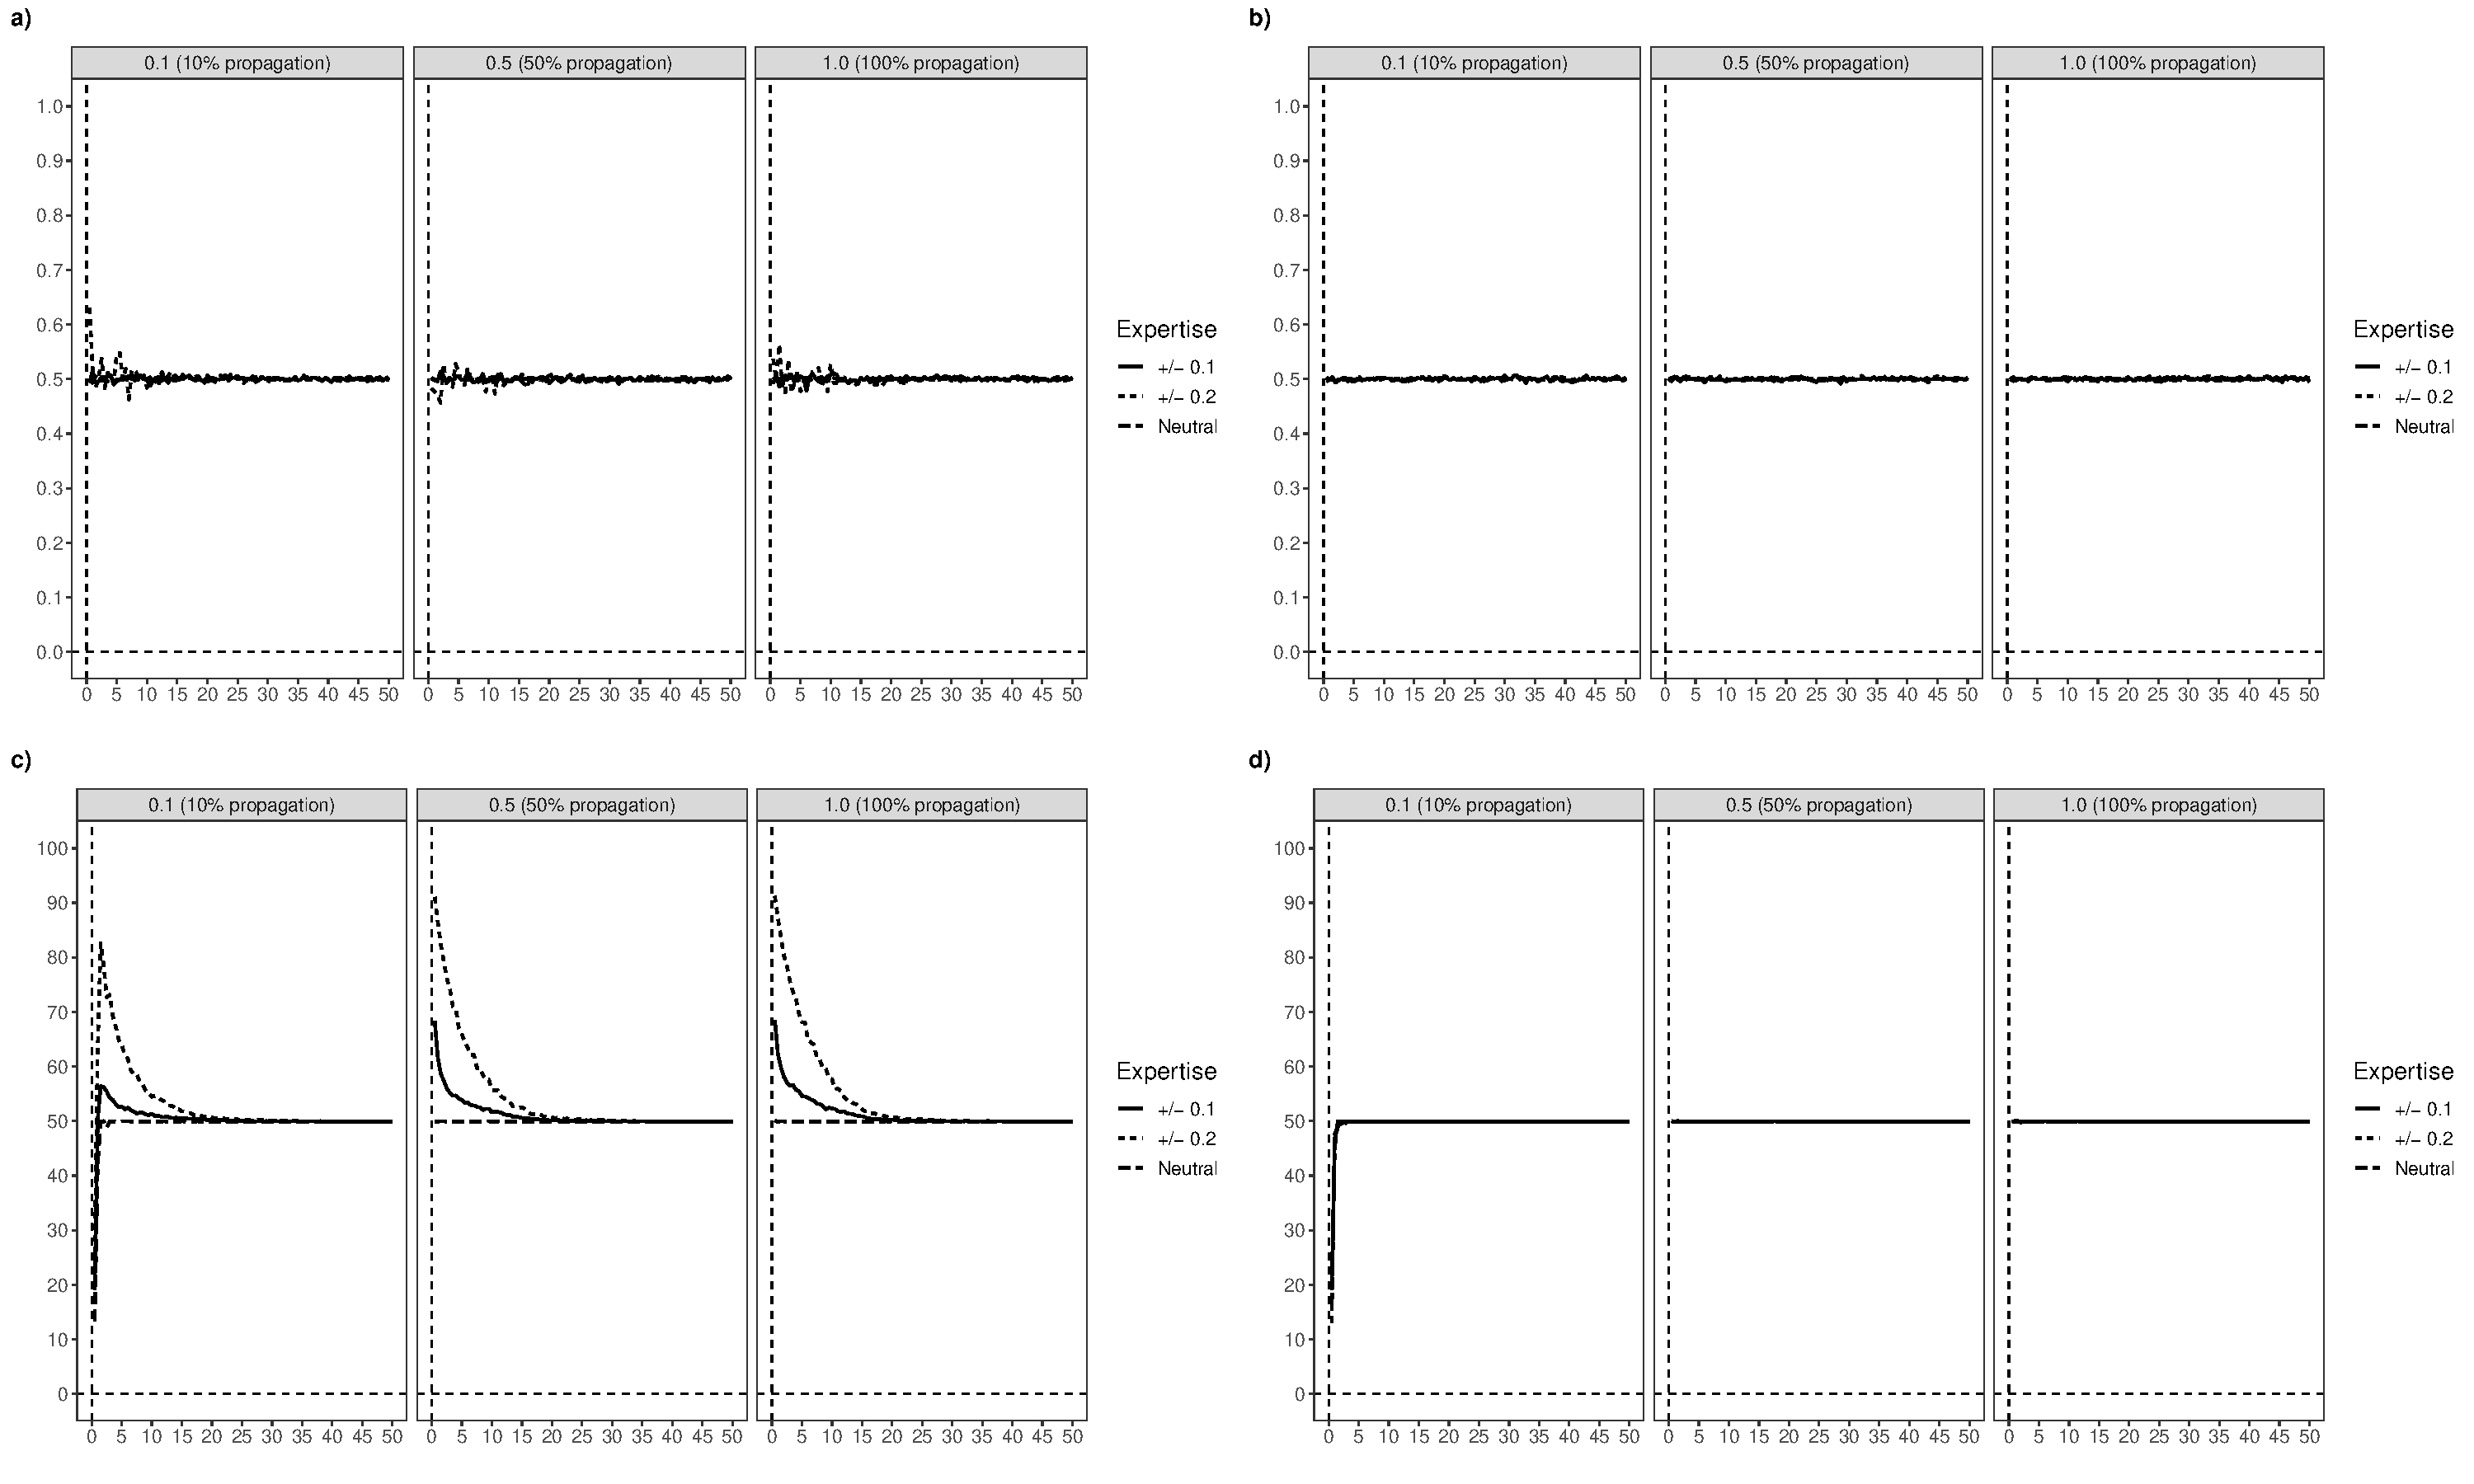
\includegraphics[width=1\columnwidth]{img/results_pdf.pdf}
%DIFDELCMD < %%%
%DIFDELCMD < \caption{%
{%DIFAUXCMD
\DIFdelFL{Main results. a) global belief proportions, social agents. b) global belief proportions, asocial agents. c) average percentage of like-minded neighbors (i.e. echo chambers), social agents. d) average percentage of like-minded neighbors (i.e. echo chambers), asocial agents.}}
%DIFAUXCMD
%DIFDELCMD < \label{fig:results}
%DIFDELCMD < \end{figure}
%DIFDELCMD < 

%DIFDELCMD < %%%
\DIFdelend The finding that an expertise strength of 0 (i.e. neutral) prevented the formation of echo chambers is a natural result of our model \DIFaddbegin \DIFadd{(robustness check 1)}\DIFaddend . Specifically, setting expertise strength to 0 reduces the communicative impact of a source to 0, irrespective of their perceived credibility (for details see Methods). Consequently, a receiver won't be influenced by the communicating source, which can conceptually be compared to disregarding the belief of a social media user that has no epistemic authority (i.e., no knowledge about the topic of discussion).

Fig. \ref{fig:results}d shows the clustering results from our asocial agent population. If agents randomly connect with their network-peers, \DIFdelbegin \DIFdel{meaning that they stochastically sampled credibility estimates for each source, }\DIFdelend no echo chambers \DIFdelbegin \DIFdel{emerged}\DIFdelend \DIFaddbegin \DIFadd{emerge}\DIFaddend . This finding highlights the \DIFdelbegin \DIFdel{importance }\DIFdelend \DIFaddbegin \DIFadd{implications of }\DIFaddend selecting network-peers based on positive credibility perceptions (e.g., friendship): while stochastic selection prevents echo chambers, selecting network peers based on whom one likes is a key requirement for echo chamber formation. 
\DIFdelbegin %DIFDELCMD < 

%DIFDELCMD < %%%
\DIFdelend The results in the left panels of Figs. \ref{fig:results}c-d (P(Declaration) = 10\%) showing a reduced clustering effect for connectivity density values of 0.5\% can be fully attributed to \DIFaddbegin \DIFadd{the effective }\DIFaddend fracturing of the network (i.e. no information cascade occurred)\DIFdelbegin \DIFdel{. This finding demonstrates that if we did not share information on social media, we would not get information cascades . }\DIFdelend \DIFaddbegin \DIFadd{, when users do not share information (robustness check 2). This demonstrates that information cascades require us to share information laterally.
}

\DIFaddend To visualise the above findings, Fig. \DIFdelbegin \DIFdel{\ref{fig:example_nets} }\DIFdelend \DIFaddbegin \DIFadd{\ref{fig:example} }\DIFaddend includes example outcomes of post-cascade belief proportions with 1\% and 5\% connectivity density. a) and c) correspond to our social agent population and b) and d) pertain to the asocial population. \DIFaddbegin \DIFadd{Red and blue colours illustrate clusters of similar-minded agents holding different beliefs. Specifically, as seen in  Fig. \ref{fig:example}a and  Fig. \ref{fig:example}c, social agents formed two polarised clusters of similar-minded agents, with limited communication between clusters. Fig. \ref{fig:example}b and  Fig. \ref{fig:example}d show the results from the asocial agent population, which did not show any signs of echo chambers. Here, most agents connected to an equal proportion of similar and dissimilar beliefs, which is illustrated by the absence of distinct colour patterns.
}\DIFaddend 


\begin{figure}[ht]
\centering
\DIFdelbeginFL %DIFDELCMD < 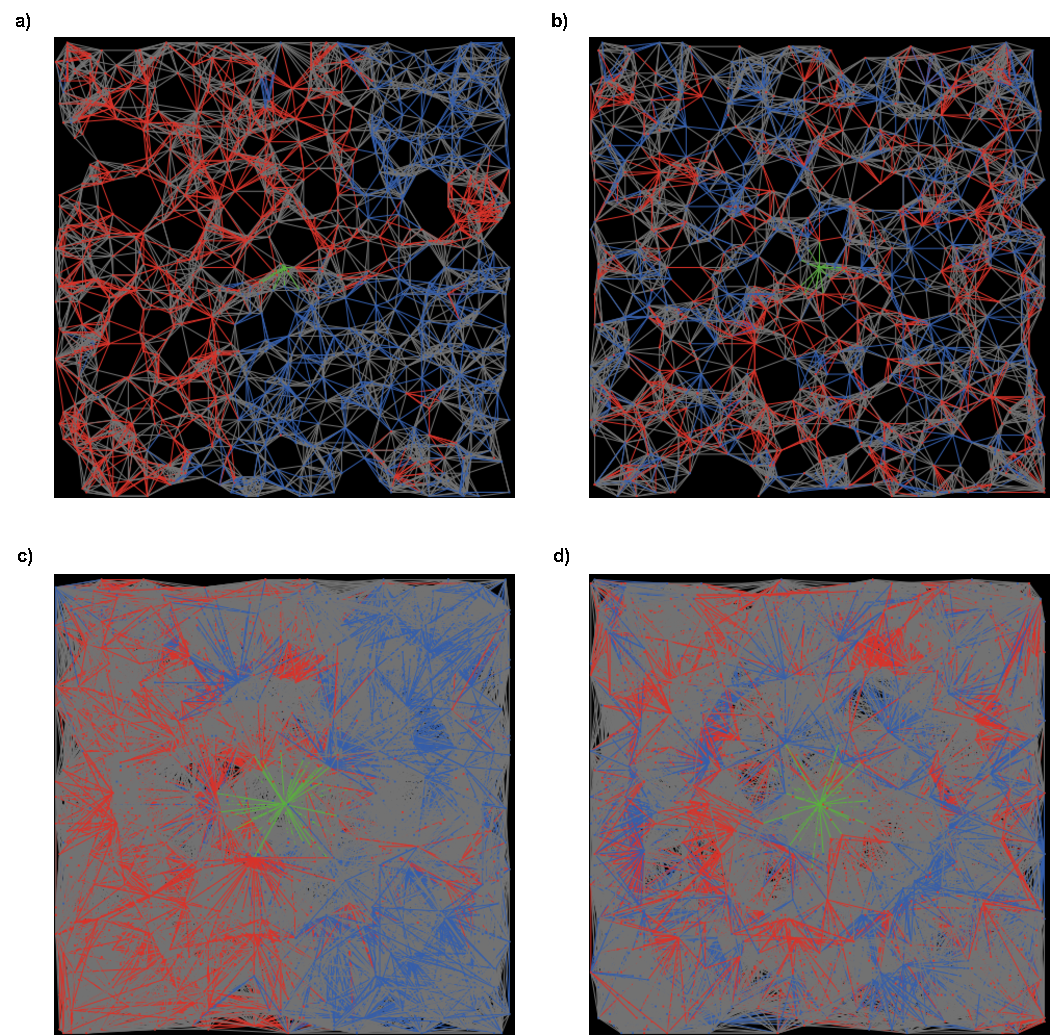
\includegraphics[width=0.8\columnwidth]{img/example_networks.pdf}
%DIFDELCMD < %%%
\DIFdelendFL \DIFaddbeginFL 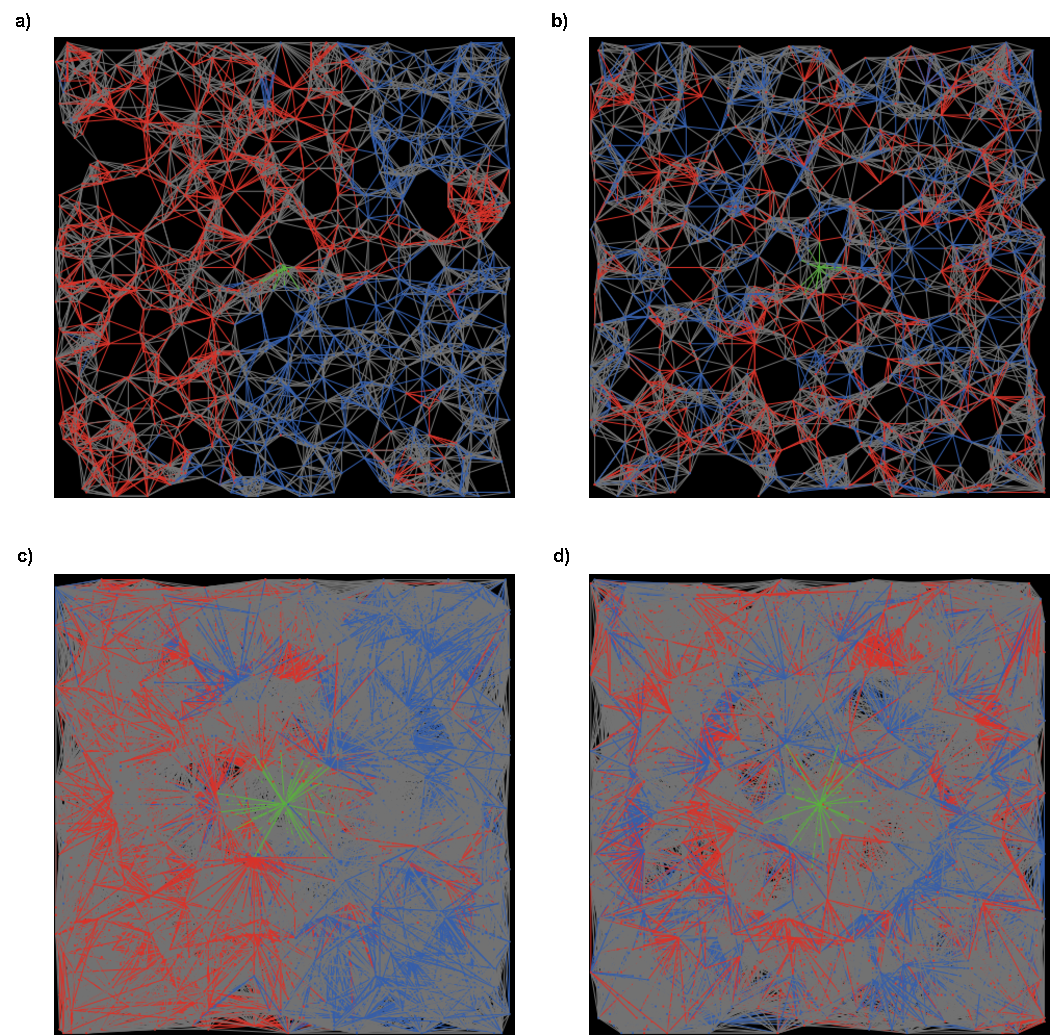
\includegraphics[width=0.8\columnwidth]{figure3.pdf}
\DIFaddendFL \caption{Example post-cascade networks. Grey = agents that did not declare a belief; blue = agents believing \(\neg h\); red = agents believing \(h\). Connectivity density values of upper networks: a) social agents: 1\%; b) asocial agents: 1\%. Connectivity density values of lower networks: c) social agents: 5\%; d) asocial agents: 5\%.}
\DIFdelbeginFL %DIFDELCMD < \label{fig:example_nets}
%DIFDELCMD < %%%
\DIFdelendFL \DIFaddbeginFL \label{fig:example}
\DIFaddendFL \end{figure}

\section*{Discussion}
The aim of this work was to disentangle previously conflated causes of echo chambers on social media. Specifically, we examined whether echo chambers emerge in a population of homogeneous, \DIFdelbegin \DIFdel{individually }\DIFdelend \DIFaddbegin \DIFadd{equally }\DIFaddend rational users that engage in a single interaction. Our results show that echo chambers emerge in \DIFdelbegin \DIFdel{a population of individually }\DIFdelend \DIFaddbegin \DIFadd{an idealised population of equally }\DIFaddend rational agents who integrate the beliefs of others with their own prior beliefs in a Bayesian manner. Moreover, we showed that echo chambers emerge through a single pass-through of information prior to repeated interaction.

These results suggest that previously identified causes of echo chambers, including psychological biases and inter-individual differences in terms of the cognitive architecture of agents, might not be necessary for the observation of echo chambers. \DIFaddbegin \DIFadd{Specifically, agents in the present model were furnished with a homogeneous cognitive architecture, meaning that they shared the same belief updating mechanisms, irrespective of their subjective prior beliefs. They also did not rewire their social ties based on a bias against agents holding different beliefs, which has been addressed in previous models of echo chambers \mbox{%DIFAUXCMD
\cite{henry2011emergence, madsen2018large, sasahara2019inevitability}}\hspace{0pt}%DIFAUXCMD
. }\DIFaddend Moreover, our findings suggest that repeated interaction, \DIFdelbegin \DIFdel{which has been }\DIFdelend a key component \DIFdelbegin \DIFdel{in previous models of echo chambers \mbox{%DIFAUXCMD
\cite{madsen2017growing, madsen2018large}}\hspace{0pt}%DIFAUXCMD
, might }\DIFdelend \DIFaddbegin \DIFadd{of previous related work \mbox{%DIFAUXCMD
\cite{madsen2017growing, madsen2018large}}\hspace{0pt}%DIFAUXCMD
, may }\DIFaddend not be required for the observation of echo chambers. \DIFaddbegin \DIFadd{More precisely, while the results of previous models have revealed that echo chambers emerge as a consequence of repeated interaction between similar-minded agents, we showed that a single interaction between generations of agents resulted in the formation of echo chambers. }\DIFaddend On average, each belief was equally represented in our simulations. Thus, our results further show that segregated groups \DIFdelbegin \DIFdel{did not evolve as }\DIFdelend \DIFaddbegin \DIFadd{were not }\DIFaddend a consequence of \DIFdelbegin \DIFdel{a }\DIFdelend global dominance of \DIFdelbegin \DIFdel{a particular }\DIFdelend \DIFaddbegin \DIFadd{one }\DIFaddend belief (see Figs. \ref{fig:results}-\DIFdelbegin \DIFdel{\ref{fig:example_nets}}\DIFdelend \DIFaddbegin \DIFadd{\ref{fig:example}}\DIFaddend ). 

Furthermore, and central to the present paper\DIFdelbegin \DIFdel{is the finding }\DIFdelend \DIFaddbegin \DIFadd{, we find }\DIFaddend that the emergence of echo chambers was confined to \DIFdelbegin \DIFdel{the social agent population }\DIFdelend \DIFaddbegin \DIFadd{populations }\DIFaddend in which network-peers were selected on the basis of positive credibility estimates. Specifically, we showed that self-selecting peers based on whom one likes \DIFdelbegin \DIFdel{(i.e. perceives positively) }\DIFdelend carries a potentially deleterious consequence for the formation of echo chambers. If network-peers \DIFdelbegin \DIFdel{are }\DIFdelend \DIFaddbegin \DIFadd{were }\DIFaddend selected at random\DIFaddbegin \DIFadd{, }\DIFaddend and thus independent of whom one likes or perceives positively (asocial agents), no echo chambers emerged. \DIFaddbegin \DIFadd{Importantly, self-selection based on positive credibility estimates is different from rewiring social ties based on a preference for beliefs. While agents in previous work  \mbox{%DIFAUXCMD
\cite{henry2011emergence, madsen2018large} }\hspace{0pt}%DIFAUXCMD
were }\emph{\DIFadd{unwilling}} \DIFadd{to exchange their beliefs with dissimilar peers, the present social agent population did not exclude peers with different beliefs from their network. Instead, they evaluated the credibility of a communicating agent (operationalised via trustworthiness and expertise) based on the beliefs of all peers in their network (see Methods, for details).
}\DIFaddend 

Overall, our findings illustrate that echo chambers, which might induce spreading and retention of misinformation\cite{vosoughi2018spread}, conspiratorial thinking\cite{del2016spreading}, and political polarisation\cite{bessi2016users, del2016echo}, are not necessarily caused by the inhabitants of social networks directly. Rather, the \textit{structure} of social networks, and notably the \DIFdelbegin \DIFdel{constraining }\DIFdelend lateral (i.e. peer-to-peer) transmission of information\DIFaddbegin \DIFadd{, }\DIFaddend can be sufficient for echo chamber formation\DIFaddbegin \DIFadd{, when a network is built on self-selecting peers}\DIFaddend . The degree of making opinions public (P(Declaration)) did affect echo chamber formation only if it was so low that it effectively fractured the functional message passing around the network. Additionally, the magnitude of expertise strength modulated the influence of credibility, resulting in increased echo chamber effects for higher levels of expertise. This suggests that being friends with expert users might exacerbate the formation of echo chambers. Given that the present simulations included rational Bayesian agents, it is further expected that incorporation of additional psychological variables, such as the confirmation bias \cite{del2016spreading, ngampruetikorn2016bias, starnini2016emergence}, might intensify the strength and persistence of echo chambers (see also \cite{pilditch2017opinion}). \DIFaddbegin \DIFadd{While these findings suggests that social networks by design might be causally sufficient for echo chamber formation, it is important that further empirical research investigates the ecological validity of our model results in real-world social networks. 
}\DIFaddend 

More generally, our results show that agent-based models, which enable capturing of dynamic interactions between individuals, provide a valuable opportunity for studying the formation of emergent phenomena such as echo chambers. This is in line with a growing body of literature employing agent-based models to investigate several related phenomena, including opinion polarisation \cite{duggins2017}, identity search \cite{watts2002identity}, \DIFdelbegin \DIFdel{disbelief }\DIFdelend \DIFaddbegin \DIFadd{(dis)belief }\DIFaddend in climate change \DIFdelbegin \DIFdel{\mbox{%DIFAUXCMD
\cite{lewandowsky2019influence} }\hspace{0pt}%DIFAUXCMD
}\DIFdelend \DIFaddbegin \DIFadd{\mbox{%DIFAUXCMD
\cite{williams2015network, lewandowsky2019influence} }\hspace{0pt}%DIFAUXCMD
}\DIFaddend and micro-targeting \cite{madsen2018method}. Given the potential of agent-based models for studying echo chambers and related emergent phenomena, it is important that further work develops interventions which might reduce the occurrence of opinion segregation. Such interventions might extend previous work suggesting that `educational broadcasts' across a network of idealised Bayesian agents (similar to the present model) reduce echo chamber formation \cite{madsen2018large}.

An important avenue for further work might be a closer examination of the belief updating process of the present agent populations. Specifically, agents in the present populations updated beliefs sequentially based on the declarations of previous generations. Recent empirical studies demonstrated that people are sensitive to such statistical dependencies in social learning. \DIFdelbegin \DIFdel{Across both abstract (e.g., estimating the number marbles in an urn; see \mbox{%DIFAUXCMD
\cite{whalen2018sensitivity} }\hspace{0pt}%DIFAUXCMD
) and more applied tasks (e.g., rating the suitability of a political candidate for public office), it has been shown that people differentiate between the evidential signal of independent beliefs and dependent beliefs that were formed sequentially. When beliefs }\DIFdelend \DIFaddbegin \DIFadd{For example, \mbox{%DIFAUXCMD
\cite{whalen2018sensitivity} }\hspace{0pt}%DIFAUXCMD
showed that when beliefs }\DIFaddend of others were formed sequentially, people updated their prior beliefs less. Considering \DIFdelbegin \DIFdel{these }\DIFdelend \DIFaddbegin \DIFadd{such }\DIFaddend findings, an important step for follow-up simulations involves testing the robustness of echo chambers between varying levels of belief dependencies in a network. \DIFdelbegin \DIFdel{Here, empirical findings by \mbox{%DIFAUXCMD
\cite{whalen2018sensitivity} }\hspace{0pt}%DIFAUXCMD
might serve as input validation for simulations, enabling agents to differentiate between independent and sequentially updated beliefs. }%DIFDELCMD < 

%DIFDELCMD < %%%
\DIFdel{In summary, while the study of echo chambers does by no means exhaustively address the issue of digital misinformation, it provides an important contribution to our understanding of how people settle on beliefs in social networks. Here, we show that echo chambers emerge as a consequence of self-selection of network peers (e. g., friends), limited access to information (i.e. local connectivity), and lateral transmission of information between social agents. This suggests that social networks by design can be causally sufficient for echo chamber formation. As a consequence, we show that previously conflated causes such as psychological biases, inter-individual differences, and repeated interaction, might not be necessary. Rather, such inter-individual differences and psychological variables, including confirmation bias, are expected to exacerbate the formation of echo chambers. Finally, we show that the computations involved in evaluating the credibility of a source play a key role in the formation of echo chambers.
Together, these findings raise questions for social network architects, and notably the potentially deleterious consequences of encouraging peer-to-peer content sharing.
}\DIFdelend \DIFaddbegin \DIFadd{An additional extension might focus on the declaration functions used prior to communicating beliefs. In the present work, agents used a deterministic decision rule. Potential alternatives that might be contrasted in future work include probability matching \mbox{%DIFAUXCMD
\cite{shanks2002re} }\hspace{0pt}%DIFAUXCMD
or the communication of full probability densities.
}\DIFaddend 

%DIF >  In summary, while the study of echo chambers does by no means exhaustively address the issue of digital misinformation, it provides an important contribution to our understanding of how people settle on beliefs in social networks. Using an idealised population of social network users, we demonstrate that echo chambers emerge as a consequence of self-selection of network peers (e.g., friends), limited access to information (i.e. local connectivity), and lateral transmission of information between social agents. 
\DIFaddbegin 

%DIF >  Thus, we show that previously conflated causes, such as psychological biases, inter-individual differences, and repeated interaction, are not strictly \textit{required} for echo chamber formation with these network structures. 

%DIF >  However, such inter-individual differences and psychological variables, including confirmation bias, are expected to exacerbate the formation of echo chambers. While these findings suggests that social networks by design can be causally sufficient for echo chamber formation, it is important that further empirical research investigates the ecological validity of our model results in real-world social networks. 

%DIF >  Finally, we show that the computations involved in evaluating the credibility of a source play a key role in the formation of echo chambers. Together, these findings raise questions for social network architects.

%DIF >  and notably the potentially deleterious consequences of encouraging peer-to-peer content sharing.


\DIFaddend \section*{Methods}

\subsection*{BSCM details}

Table \ref{tab:t2} shows the conditional probability table which specified how the different components of the likelihood were computed. To ensure that the direction of the influence of expertise strength (\(\textbf{\textit{e}}\)) matched an agent's prior belief (i.e. towards 1 if \(P(h)\) > 0.5 and towards 0 if  \(P(h)\) < 0.5), we flipped the impact of expertise strength based on the prior. Similar to an indicator function, \(\textbf{\emph{I}}\) thus returned 1 for agents having a prior belief \(P(h)\) > 0.5 and -1 for agents having a prior belief \(P(h)\) < 0.5. \(\tau\) is an additional constant that quantifies the presence vs. absence of expertise. Manipulating values of \(\tau\) results in stronger differences between varying levels of expertise strength. For all simulations, \(\tau\) = 2, meaning that the magnitude of belief change for a medium expert (i.e.  (\(\textbf{\textit{e}}\)) = 0.1) ranged from -0.2 to 0.2 while the magnitude for a high expert (i.e.  (\(\textbf{\textit{e}}\)) = 0.2) ranged from -0.4 to 0.4. For  \(\textbf{\textit{e}}\) = 0, there was no effect on belief change. 

\begin{table}[ht]
\label{tab:bscm_details}
\centering
\DIFdelbeginFL %DIFDELCMD < \begin{tabular}{|l|l|l|1|1|}
%DIFDELCMD < %%%
\DIFdelendFL \DIFaddbeginFL \begin{tabular}{|c|c|c|c|c|c}

\DIFaddendFL \hline
& e, t & \DIFdelbeginFL \DIFdelFL{\neg }\DIFdelendFL \DIFaddbeginFL \DIFaddFL{\(\neg\)}\DIFaddendFL e, t & e, \DIFdelbeginFL \DIFdelFL{\neg }\DIFdelendFL \DIFaddbeginFL \DIFaddFL{\(\neg\)}\DIFaddendFL t & \DIFdelbeginFL \DIFdelFL{\neg e,\neg }\DIFdelendFL \DIFaddbeginFL \DIFaddFL{\(\neg\)e,\(\neg\)}\DIFaddendFL t\\
\hline
h & 0.5 + eI\DIFdelbeginFL \DIFdelFL{_{P(h)>0.5}*\tau }\DIFdelendFL \DIFaddbeginFL \DIFaddFL{\(_{P(h)>0.5}\)\(\times\)\(\tau\) }\DIFaddendFL & 0.5 + eI\DIFdelbeginFL \DIFdelFL{_{P(h)>0.5} }\DIFdelendFL \DIFaddbeginFL \DIFaddFL{\(_{P(h)>0.5}\) }\DIFaddendFL & 0.5 - eI\DIFdelbeginFL \DIFdelFL{_{P(h)>0.5}*\tau  }\DIFdelendFL \DIFaddbeginFL \DIFaddFL{\(_{(P(h)>0.5}\)\(\times\)\(\tau\) }\DIFaddendFL &  0.5 - eI\DIFdelbeginFL \DIFdelFL{_{P(h)>0.5}}\DIFdelendFL \DIFaddbeginFL \DIFaddFL{\(_{(P(h)>0.5}\)}\DIFaddendFL \\
\DIFaddbeginFL 

\DIFaddendFL \hline
\DIFdelbeginFL \DIFdelFL{\neg }\DIFdelendFL \DIFaddbeginFL \DIFaddFL{\(\neg\)}\DIFaddendFL h & 1 - (0.5 + eI\DIFdelbeginFL \DIFdelFL{_{P(h)>0.5}*\tau}\DIFdelendFL \DIFaddbeginFL \DIFaddFL{\(_{P(h)>0.5}\)\(\times\)\(\tau\)}\DIFaddendFL ) & 1 - (0.5 + eI\DIFdelbeginFL \DIFdelFL{_{P(h)>0.5}}\DIFdelendFL \DIFaddbeginFL \DIFaddFL{\(_{P(h)>0.5}\)}\DIFaddendFL ) & 1 - (0.5 - eI\DIFdelbeginFL \DIFdelFL{_{P(h)>0.5}*\tau}\DIFdelendFL \DIFaddbeginFL \DIFaddFL{\(_{P(h)>0.5}\)\(\times\)\(\tau\)}\DIFaddendFL ) & 1 - (0.5 - eI\DIFdelbeginFL \DIFdelFL{_{P(h)>0.5}}\DIFdelendFL \DIFaddbeginFL \DIFaddFL{\(_{P(h)>0.5}\)}\DIFaddendFL )\\
\DIFaddbeginFL 

\DIFaddendFL \hline
\end{tabular}
\caption{\label{tab:t2}Conditional probability table.}
\end{table}


The BSCM architecture provides a general framework for updating one's belief under consideration of a source's credibility. It does not specify how individual agents estimate the perceived expertise and perceived trustworthiness values of a source during interaction. Here, we refer to an important element of social networks: selecting network-peers on the basis of whom one likes (i.e. positive credibility estimates). We operationalised this self-selection property in a hypothetical population of `social agents' who weigh the perceived credibility of a communicating source based on the beliefs of their peers. Specifically, following observation of a source's belief in a hypothesis, a target agent (receiver) weighs the expertise and trustworthiness of a communicating source based on the proportion of agents in the receiver's direct network entertaining the same belief as the source and the number of agents in the network entertaining the opposite belief of the source. More formally, this can be written as  

\begin{equation}
    \DIFdelbegin \DIFdel{P(}\DIFdelend e\DIFdelbegin \DIFdel{) }\DIFdelend \DIFaddbegin \DIFadd{_{com} }\DIFaddend = \frac{\sum_{i=1}^{N_h}e_i}{\sum_{i=1}^{N_h}e_i + \sum_{i=1}^{N_{\neg h}}e_i}          
\end{equation}

\begin{equation}
    \DIFdelbegin \DIFdel{P(}\DIFdelend t\DIFdelbegin \DIFdel{) }\DIFdelend \DIFaddbegin \DIFadd{_{com} }\DIFaddend = \frac{\sum_{i=1}^{N_h}t_i}{\sum_{i=1}^{N_h}t_i + \sum_{i=1}^{N_{\neg h}}t_i}
\end{equation}
\DIFdelbegin %DIFDELCMD < 

%DIFDELCMD < %%%
\DIFdel{where \(e\) and \(t\) }\DIFdelend \DIFaddbegin \DIFadd{where \(e_{com}\) and \(t_{com}\) }\DIFaddend correspond to the \DIFdelbegin \DIFdel{subjective estimates for individual agents in the receiver's network (sampled from univariate Gaussians with \(\mu\)=0.5 and \(\sigma^2\)=0.20; see Fig. \ref{fig:bscm} for an illustration) }\DIFdelend \DIFaddbegin \DIFadd{specific (weighted) credibility estimates that a communication target assigns to a communicating source}\DIFaddend .

% (which is a function of the weighted proportion of agents supporting the same belief as the source compared to the total number of believers in a receiver's network).

We contrasted the above population of social agents with a second population of asocial agents in which connections with peers were established at random. Random selection of peers was operationalised by random sampling of perceived expertise and perceived trustworthiness of sources from a uniform distribution bounded between [0, 1]. This means that asocial agents computed stochastic credibility estimates for a source irrespective of the beliefs of their network peers. Asocial agents thus enabled to assess the relevance of selecting network-peers based on positive credibility estimates of others / friendship. For simulations across both hypothetical populations (social and asocial), \DIFdelbegin \DIFdel{perceived expertise \(P(e)\) and trustworthiness \(P(t)\) }\DIFdelend \DIFaddbegin \DIFadd{the weighted expertise \(e_{com}\) and trustworthiness \(t_{com}\) }\DIFaddend estimates were plugged into Equations 2-3 to \DIFdelbegin \DIFdel{compute the likelihood of observing a source's beliefgiven the receivers prior belief }\DIFdelend \DIFaddbegin \DIFadd{replace \(P(e)\) }\DIFaddend and \DIFdelbegin \DIFdel{the credibility of the source. }\DIFdelend \DIFaddbegin \DIFadd{\(P(t)\), respectively. 
%DIF >  the likelihood of observing a source's belief given the receivers prior belief and the credibility of the source.
}\DIFaddend 

\DIFdelbegin \subsection*{\DIFdel{More on simulations}}
%DIFAUXCMD
\DIFdelend \DIFaddbegin \subsection*{\DIFadd{Agent-based models and simulations}}
\DIFadd{The three central components of ABMs are agents, patches, and links. Agents are the actors, and in our social network they correspond to individual users. Agents were furnished with cognitive functions and possible behaviours, including attention (detecting public declarations of others), belief revision (updating a prior belief-state based on observing another agent’s belief), and declaration (commit to a belief using a decision rule). All agents were furnished with the same cognitive functions and possible behaviours. Links represent edges between agents. In the present model, bidirectional links were employed to enable signaling of public belief declarations between agents. Links thus represent the (social) network connections between users. Patches are the building blocks of the environment in which agents act. For example, patches can represent trees in a forest or the number of fish in a specific location of a lake. Agents can interact with patches---if agents were fishermen, they could move around and fish from specific locations \mbox{%DIFAUXCMD
\cite{bailey2018computational}}\hspace{0pt}%DIFAUXCMD
. For the present model, patches have no further relevance as there is no interaction between agents and patches. Specifically, our simulations are confined to the cognitive architecture and belief states of agents, and all relevant interactions occur on an agent-to-agent-level.
}\DIFaddend The model was implemented in NetLogo version 6.0.4 \cite{wilensky1999netlogo}. All simulations were performed in R using the package {\tt RNetLogo()} \cite{thiele2014r}. \DIFaddbegin \DIFadd{Each system specification (connectivity density (100) x expertise strength (3) x P(Declaration) (3)) was ran independently 50 times, taking an average set of values for each specification. The total number of agents (n = 1000) was consistent across simulations. Simulations were conducted independently for each of the two agent populations.
}

\DIFaddend In the following, we outline the basic technical details of our model. Algorithm \ref{alg:al1} shows the setup procedure of the network, including placing agents in space, sampling prior \(P(h)\), \(e\), and \(t\) values, and forming connections with peers based on proximity as measured by Euclidean distance (a proxy for relational proximity in social networks; see \cite{duggins2017}). \DIFdelbegin %DIFDELCMD < 

%DIFDELCMD < \begin{algorithm}[H]
%DIFDELCMD < %%%
%DIFDELCMD < \caption{%
{%DIFAUXCMD
\DIFdel{Setup network}}%DIFAUXCMD
%DIFDELCMD < \label{setup}
%DIFDELCMD < \begin{algorithmic}[1]
%DIFDELCMD <   \Procedure{Place agents}{}
%DIFDELCMD <    \label{alg:al1}
%DIFDELCMD <     \State %%%
\DIFdel{Create $N$ agents
    }%DIFDELCMD < \For{$i=1$ to $N$}
%DIFDELCMD <         \State %%%
\DIFdel{set i position random }\DIFdelend \DIFaddbegin \DIFadd{Specifically, each agent was randomly assigned to a }\DIFaddend x-y coordinate \DIFdelbegin %DIFDELCMD < \EndFor
%DIFDELCMD <   \EndProcedure
%DIFDELCMD <   \Procedure{Setup priors and Links}{}
%DIFDELCMD <     \For{$i=1$ to $N$}
%DIFDELCMD <       \State %%%
\DIFdel{$P(h)[i]\gets x$}%DIFDELCMD < \thicksim%%%
\DIFdel{$N(\mu, \sigma^2)$ 
      }%DIFDELCMD < \State %%%
\DIFdel{$e[i]\gets x$}%DIFDELCMD < \thicksim%%%
\DIFdel{$N(\mu, \sigma^2)$
      }%DIFDELCMD < \State %%%
\DIFdel{$t[i]\gets x$}%DIFDELCMD < \thicksim%%%
\DIFdel{$N(\mu, \sigma^2)$
      }%DIFDELCMD < \State %%%
\DIFdel{create links with $n$ nearest neighbors }%DIFDELCMD < \Comment{based on Euclidean distance}
%DIFDELCMD <      \EndFor
%DIFDELCMD <   \EndProcedure
%DIFDELCMD < \end{algorithmic}
%DIFDELCMD < \end{algorithm}
%DIFDELCMD < %%%
\DIFdelend \DIFaddbegin \DIFadd{in a two-dimensional environment. After all agents were allocated to a position in space, each agent formed \(n\) bidirectional ties with other agents that were closest as measured by Euclidean distance. This means that ties between agents were formed at random and irrespective of subsequent beliefs of agents. Additionally, ties were static, meaning that after having established all connections between agents, the network structure did not change during subsequent simulations.  
}\DIFaddend 

Simulations were initiated through a neutral event node. Neutral in this case means that the first agent sampled randomly from the set of beliefs \{\(h\), \(\neg h\)\} each time it communicated to a target. Due to this stochastic process, on average, half of the \(1\textsuperscript{st}\) generation agents receiving input from the neutral event node should arrive at belief \(h\) while the other half will arrive at belief \(\neg h\) after BSCM integration. Specifically, this included attending to the declared beliefs of the neutral event node, revising initial beliefs based on the perceived credibility of the neutral event node, and deciding whether to declare an opinion public according to P(Declaration).


\DIFaddbegin \begin{algorithm}[H]
\caption{\DIFadd{Setup network}}\label{setup}
\begin{algorithmic}[1]
  \Procedure{Place agents}{}
   \label{alg:al1}
    \State \DIFadd{Create $N$ agents
    }\For{$i=1$ to $N$}
        \State \DIFadd{set i position random x-y coordinate
     }\EndFor
  \EndProcedure
  \Procedure{Setup priors and Links}{}
    \For{$i=1$ to $N$}
      \State \DIFadd{\(P(h)[i]\)\(\gets\)X$\sim$N(\(\mu\), \(\sigma\)\(^2\))
      }\State \DIFadd{\(e[i]\)\(\gets\)X$\sim$N(\(\mu\), \(\sigma\)\(^2\))
      }\State \DIFadd{\(t[i]\)\(\gets\)X$\sim$N(\(\mu\), \(\sigma\)\(^2\))
      }\State \DIFadd{create links with $n$ nearest neighbours }\Comment{based on Euclidean distance}
     \EndFor
  \EndProcedure
\end{algorithmic}
\end{algorithm}

\DIFaddend The number of agents the neutral event node communicated to was determined by the connectivity density. Connectivity values above 50\% were omitted as this would have enabled every other agent to be connected to the neutral event node in the 1st generation, precluding the occurrence of a cascade. To improve the readability of plotted example networks (Fig. \DIFdelbegin \DIFdel{\ref{fig:example_nets}}\DIFdelend \DIFaddbegin \DIFadd{\ref{fig:example}}\DIFaddend ), the initial neutral event node was  placed in the center of each simulation (i.e. central x-y-coordinate).

After revising their prior beliefs, the first-generation agents (those that received input from the neutral event node) made their beliefs public based on the manipulated P(Declaration) value. Their communication targets (i.e. second-generation) then used the communicated opinion of the first-generation agents as input for their own belief revision following the same procedure. Algorithm \ref{alg:al2} shows the basic steps involved in a single instance of belief revision (i.e. from one generation to the the next). Here, source refers to an agent from the previous generation that already publicly declared a belief (i.e. \(h\) or \(\neg h\)) and the connections of the source refer to the potential communication targets of the next generation. As we investigated whether a single pass-through of information (i.e. single interaction) was sufficient for the formation of echo chambers, we did not allow for repeated interaction, meaning that agents could not qualify as communication targets after declaring for a belief. 

\begin{algorithm}[H]
\caption{Updating beliefs}\label{update}
\begin{algorithmic}[1]
  \Procedure{Source selects communication target}{}
    \DIFdelbegin %DIFDELCMD < 

%DIFDELCMD <     %%%
\DIFdelend \If{matchCounter $\leq$ 1}
     \label{alg:al2}
        \For{$i=1$ to $n_{source}$}\Comment{n = source's connections}
            \If{i = neutral}\Comment{check if target did not already declare a belief}
             \State belief[i] = BSCM(source, n[i])\Comment{n = target's connections}
              \If{random(0.01,1.00) > P(Declaration)}
              \State propagate belief to next generation
              \EndIf
             \EndIf
        \EndFor
    \EndIf
  \EndProcedure
\end{algorithmic}
\end{algorithm}

The process of transmitting beliefs continued down successive generations until the network was either completely saturated (i.e. all agents committed to a belief) or the number of believers (i.e. \(h\) or \(\neg h\)) did not change for two consecutive time periods. Algorithm \ref{alg:al3} illustrates how this procedure was implemented in our model.

\begin{algorithm}[H]
\caption{Stop simulation}\label{proceed}
\begin{algorithmic}[1]
  \Procedure{Check if network is saturated or fractured}{}
    \State matchCounter = 0 \Comment{counts how often no change occurred between generations}
    \State Count\DIFdelbegin \DIFdel{_{\(h\)} }\DIFdelend \DIFaddbegin \DIFadd{\(_{h}\) }\DIFaddend = 0
     \label{alg:al3}
    \State Count\DIFdelbegin \DIFdel{_{\(\neg h\)} }\DIFdelend \DIFaddbegin \DIFadd{\(_{\neg h}\) }\DIFaddend = 0
    \For{$i=1$ to $N$}\Comment{N = all agents}
        \If{belief[i] = \(h\)}
            \State Count\DIFdelbegin \DIFdel{_{\(h\)} }\DIFdelend \DIFaddbegin \DIFadd{\(_{h}\) }\DIFaddend = Count\DIFdelbegin \DIFdel{_{\(h\)} }\DIFdelend \DIFaddbegin \DIFadd{\(_{h}\) }\DIFaddend + 1
        \EndIf
        \If{belief[i] = \(\neg h\)}
            \State Count\DIFdelbegin \DIFdel{_{\(\neg h\)} }\DIFdelend \DIFaddbegin \DIFadd{\(_{\neg h}\) }\DIFaddend = Count\DIFdelbegin \DIFdel{_{\(\ \)} }\DIFdelend \DIFaddbegin \DIFadd{\(_{\neg h }\) }\DIFaddend + 1
        \EndIf
    \EndFor
    \DIFdelbegin %DIFDELCMD < \If{Count_{\(h\)} = Count_{\(\neg h\)}}
%DIFDELCMD <         %%%
\DIFdelend \DIFaddbegin \If{Count\(_{h}\) = Count\(_{\neg h}\)}
        \DIFaddend \State matchCounter = matchCounter + 1
    \EndIf
  \EndProcedure
\end{algorithmic}
\end{algorithm}


\bibliography{refs}


\section*{Acknowledgements}
We would like to thank \DIFaddbegin \DIFadd{Neil R. Bramley and }\DIFaddend Jens Koed Madsen for \DIFaddbegin \DIFadd{their valuable }\DIFaddend feedback and comments. 

\section*{Author contributions statement}
J.-P.F. and T.D.P. designed research; J.-P.F. and T.D.P developed the agent-based model and conducted simulations; J.-P.F. and T.D.P. wrote the paper.

\section*{Additional information}

\textbf{Competing interests}: The authors declare no competing interests. 

\noindent{\textbf{Data availability}: The model and data sets generated and analysed during the current study will be available in the accompanying \href{https://github.com/janphilippfranken/information_cascades_jpf_tdp_2020}{GitHub} repository.}


\end{document}